\documentclass[a4paper,12pt]{article}
% --- GÓI TIẾNG VIỆT VÀ TOÁN HỌC ---
\usepackage{vntex}
\usepackage[utf8]{vietnam}
\usepackage{amsmath, amssymb, amsthm, amsfonts}

\usepackage[T1]{fontenc}
\usepackage[utf8]{inputenc}
\usepackage[vietnamese]{babel}

% --- CĂN LỀ CHUẨN BÁO CÁO ---
\usepackage[a4paper, top=2.5cm, bottom=2.5cm, left=3cm, right=2.5cm]{geometry}

% --- FONT VÀ HIỂN THỊ TOÁN ---
\usepackage{mathptmx}
\usepackage{noto}

% --- GÓI BẢNG VÀ DANH SÁCH ---
\usepackage{booktabs}
\usepackage{enumitem}

% --- HIỂN THỊ CODE, BOX, VẼ HÌNH ---
\usepackage{listings}
\usepackage[many]{tcolorbox}
\usepackage{tikz}
\usepackage{xcolor}
\usepackage{graphicx} % Thêm gói graphicx để hỗ trợ \includegraphics
\tcbuselibrary{skins, breakable}

% --- CẤU HÌNH TikZ ---
\tikzstyle{vertex}=[circle, draw, inner sep=0pt, minimum size=6pt]
\newcommand{\vertex}{\node[vertex]}

% Gói cho siêu liên kết
\usepackage{hyperref}
\hypersetup{
    colorlinks=true,
    linkcolor=blue,
    filecolor=magenta,      
    urlcolor=cyan,
    pdftitle={Project 4: Graph & Tree Traversing Problems},
    pdfpagemode=FullScreen,
}

%=============== CÁC TÙY CHỈNH VÀ ĐỊNH NGHĨA MỚI ===============

% Định nghĩa một môi trường hộp cho đề bài
\newtcolorbox{problembox}[1]{
    colback=cyan!5!white,
    colframe=cyan!75!black,
    fonttitle=\bfseries,
    title=#1,
    breakable,
    arc=4mm,
    outer arc=4mm
}

% Cấu hình định dạng cho code C++
\definecolor{codegreen}{rgb}{0,0.6,0}
\definecolor{codegray}{rgb}{0.5,0.5,0.5}
\definecolor{codepurple}{rgb}{0.58,0,0.82}
\definecolor{backcolour}{rgb}{0.95,0.95,0.95}

\lstdefinestyle{cppstyle}{
    backgroundcolor=\color{backcolour},   
    commentstyle=\color{codegreen},
    keywordstyle=\color{blue},
    numberstyle=\tiny\color{codegray},
    stringstyle=\color{codepurple},
    basicstyle=\footnotesize\ttfamily,
    breakatwhitespace=false,         
    breaklines=true,                 
    captionpos=b,                    
    keepspaces=true,                 
    numbers=left,                    
    numbersep=5pt,                  
    showspaces=false,                
    showstringspaces=false,
    showtabs=false,                  
    tabsize=2,
    language=C++
}

% Cấu hình định dạng cho code Python
\lstdefinestyle{pythonstyle}{
    backgroundcolor=\color{backcolour},
    commentstyle=\color{codegreen},
    keywordstyle=\color{magenta},
    numberstyle=\tiny\color{codegray},
    stringstyle=\color{blue},
    basicstyle=\footnotesize\ttfamily,
    breakatwhitespace=false,
    breaklines=true,
    captionpos=b,
    keepspaces=true,
    numbers=left,
    numbersep=5pt,
    showspaces=false,
    showstringspaces=false,
    showtabs=false,
    tabsize=2,
    language=Python
}

% --- BẮT ĐẦU TÀI LIỆU ---
\begin{document}

\title{Báo Cáo Cuối kỳ Môn Tổ Hợp Và Lý Thuyết Đồ Thị \newline Project 4: Graph \& Tree Traversing Problems}
\author{Trần Mạnh Đức}
\date{\today}
\maketitle


\thispagestyle{empty}
\newpage

\tableofcontents
\newpage

% =========================================================================
% ==                 PHẦN I: BIỂU DIỄN VÀ CHUYỂN ĐỔI                    ==
% =========================================================================
\section{Bài toán 4: Chuyển đổi giữa các Dạng Biểu diễn Đồ thị và Cây}
\begin{problembox}{Đề bài 4}
    Viết chương trình C/C++, Python chuyển đổi giữa 4 dạng biểu diễn: adjacency matrix, adjacency list, extended adjacency list, adjacency map cho 3 đồ thị: đơn đồ thị, đa đồ thị, đồ thị tổng quát; \& 3 dạng biểu diễn: array of parents, first-child next-sibling, graph-based representation of trees của cây.

    Sẽ có $3 A_4^2 + A_3^2 = 3 \times 12 + 6 = 42$ converter programs.
\end{problembox}

\subsection{Phân tích Yêu cầu và Chiến lược Thực hiện}
Bài toán yêu cầu xây dựng một bộ công cụ toàn diện để chuyển đổi qua lại giữa các cách biểu diễn khác nhau của đồ thị và cây.


\subsubsection{Chiến lược Thiết kế: Sử dụng một ``Cấu trúc Trung gian''}
Thay vì viết tất cả 42 hàm chuyển đổi trực tiếp (ví dụ: Matrix $\to$ Map, List $\to$ Matrix, v.v.), một chiến lược hiệu quả hơn nhiều là chọn ra một \textbf{cấu trúc biểu diễn trung gian (intermediate representation)} và viết các hàm chuyển đổi từ mọi dạng khác sang dạng trung gian này, và ngược lại.

\begin{itemize}
    \item \textbf{Dạng trung gian được chọn cho Đồ thị:} Một danh sách tất cả các cạnh \texttt{(u, v, weight)}. Đây là dạng biểu diễn đơn giản, không cấu trúc, chứa tất cả thông tin cần thiết.
    \item \textbf{Dạng trung gian được chọn cho Cây:} Một danh sách các cạnh có hướng \texttt{(parent, child)} và một biến để lưu đỉnh gốc (root).
\end{itemize}
Với chiến lược này, thay vì $N \times (N-1)$ hàm, ta chỉ cần $2 \times N$ hàm để có thể chuyển đổi giữa mọi cặp.

\subsection{Thiết kế Cấu trúc Dữ liệu}
Để nhất quán, chúng ta sẽ định nghĩa các cấu trúc dữ liệu trong C++ và Python.

\subsubsection{Cấu trúc Dữ liệu C++}
\begin{lstlisting}[style=cppstyle, caption={Định nghĩa các cấu trúc dữ liệu biểu diễn đồ thị trong C++.}, label={lst:cpp_structures_4}]
#include <vector>
#include <list>
#include <map>
#include <optional> // For optional values

// A simple struct to represent an edge, our intermediate representation
struct Edge {
    int u;
    int v;
    int weight = 1; // Default weight
};

// 1. Adjacency Matrix
// For a weighted graph, value is weight. For unweighted, 1 if edge exists, 0 otherwise.
// An optional<int> can represent no edge (std::nullopt).
using AdjacencyMatrix = std::vector<std::vector<std::optional<int>>>;

// 2. Adjacency List (suitable for simple graphs and multigraphs)
// The pair stores {neighbor, weight}.
using AdjacencyList = std::vector<std::vector<std::pair<int, int>>>;

// 3. Extended Adjacency List (explicit edges)
// Not commonly used, often class-based. For simplicity, we can define it
// as a pair of incoming and outgoing adjacency lists.
struct ExtAdjList {
    AdjacencyList outgoing;
    AdjacencyList incoming;
};

// 4. Adjacency Map
// More flexible than vector for sparse graphs or non-integer vertices.
// Maps a node to a map of its neighbors and the edge weight.
using AdjacencyMap = std::map<int, std::map<int, int>>;

// --- Tree Representations ---
// 1. Array of Parents
// Index is the child node, value is the parent node. Root's parent is -1.
using ArrayOfParents = std::vector<int>;

// 2. First-Child, Next-Sibling
struct FCNS_Node { int first_child = -1; int next_sibling = -1; };
using FCNS_Representation = std::vector<FCNS_Node>;

// 3. Graph-based Representation
// A tree is a special case of a graph, so AdjacencyList can be used.
\end{lstlisting}

\subsubsection{Cấu trúc Dữ liệu Python}
\begin{lstlisting}[style=pythonstyle, caption={Định nghĩa các cấu trúc dữ liệu biểu diễn đồ thị trong Python.}, label={lst:py_structures_4}]
# Intermediate representation: A list of tuples [(u, v, weight), ...]
EdgeList = list[tuple[int, int, int]]

# 1. Adjacency Matrix
# A list of lists. None or 0 can represent no edge.
AdjacencyMatrix = list[list[int | None]]

# 2. Adjacency List (for multigraphs/general graphs)
# A dictionary mapping a node to a list of (neighbor, weight) tuples.
AdjacencyList = dict[int, list[tuple[int, int]]]

# 3. Adjacency Map (for simple graphs)
# A dictionary mapping a node to another dictionary of {neighbor: weight}.
AdjacencyMap = dict[int, dict[int, int]]

# 4. Extended Adjacency List (Conceptual)
# Can be represented as a dictionary with 'incoming' and 'outgoing' keys.
ExtendedAdjacencyList = dict[str, AdjacencyList]

# --- Tree Representations ---
# 1. Array of Parents
# A list where index is child and value is parent.
ArrayOfParents = list[int]

# 2. First-Child, Next-Sibling
# A list of dictionaries, e.g., [{'first_child': -1, 'next_sibling': -1}, ...]
FCNS_Representation = list[dict[str, int]]
\end{lstlisting}

\subsection{Cài đặt các Hàm Chuyển đổi (Python)}
Dưới đây là mã nguồn Python đầy đủ cho các bộ chuyển đổi, sử dụng danh sách cạnh làm cấu trúc trung gian.

\begin{lstlisting}[style=pythonstyle, caption={Bộ chuyển đổi đồ thị và cây trong Python.}, label={lst:py_converters_4}]
# --- Graph Converters ---

def edge_list_to_adj_matrix(edge_list: EdgeList, num_nodes: int) -> AdjacencyMatrix:
    matrix = [[None] * num_nodes for _ in range(num_nodes)]
    for u, v, weight in edge_list:
        # For simple graphs, this would overwrite. For multigraphs, it keeps the last seen edge.
        # A better approach for multigraphs would be to store min weight.
        matrix[u][v] = weight
    return matrix

def adj_matrix_to_edge_list(matrix: AdjacencyMatrix) -> EdgeList:
    edge_list = []
    num_nodes = len(matrix)
    for i in range(num_nodes):
        for j in range(num_nodes):
            if matrix[i][j] is not None:
                edge_list.append((i, j, matrix[i][j]))
    return edge_list

def edge_list_to_adj_list(edge_list: EdgeList, num_nodes: int) -> AdjacencyList:
    adj_list = {i: [] for i in range(num_nodes)}
    for u, v, weight in edge_list:
        adj_list[u].append((v, weight))
    return adj_list

def adj_list_to_edge_list(adj_list: AdjacencyList) -> EdgeList:
    edge_list = []
    for u, neighbors in adj_list.items():
        for v, weight in neighbors:
            edge_list.append((u, v, weight))
    return edge_list

def edge_list_to_adj_map(edge_list: EdgeList) -> AdjacencyMap:
    adj_map = {}
    for u, v, weight in edge_list:
        if u not in adj_map:
            adj_map[u] = {}
        # This naturally handles simple graphs (overwrites)
        adj_map[u][v] = weight
    return adj_map
    
def adj_map_to_edge_list(adj_map: AdjacencyMap) -> EdgeList:
    edge_list = []
    for u, neighbors in adj_map.items():
        for v, weight in neighbors.items():
            edge_list.append((u, v, weight))
    return edge_list

# Note: Extended Adjacency List converters would be combinations of the above.

# --- Tree Converters ---
# Intermediate representation: edge list and a root node index.

def array_of_parents_to_tree_edges(parents: ArrayOfParents) -> tuple[EdgeList, int]:
    edges = []
    root = -1
    for i, p in enumerate(parents):
        if p != -1:
            edges.append((p, i, 1)) # Assuming unweighted tree
        else:
            root = i
    return edges, root

def tree_edges_to_array_of_parents(edges: EdgeList, num_nodes: int) -> ArrayOfParents:
    parents = [-1] * num_nodes
    for p, c, _ in edges:
        parents[c] = p
    return parents

def tree_edges_to_fcns(edges: EdgeList, num_nodes: int) -> FCNS_Representation:
    children_list = [[] for _ in range(num_nodes)]
    for p, c, _ in edges:
        children_list[p].append(c)

    fcns = [{'first_child': -1, 'next_sibling': -1} for _ in range(num_nodes)]
    for i in range(num_nodes):
        if children_list[i]:
            fcns[i]['first_child'] = children_list[i][0]
            for j in range(len(children_list[i]) - 1):
                current_child = children_list[i][j]
                next_child = children_list[i][j+1]
                fcns[current_child]['next_sibling'] = next_child
    return fcns

def fcns_to_tree_edges(fcns: FCNS_Representation) -> tuple[EdgeList, int]:
    edges = []
    is_child = [False] * len(fcns)
    for parent_idx, node_data in enumerate(fcns):
        child = node_data['first_child']
        while child != -1:
            edges.append((parent_idx, child, 1))
            is_child[child] = True
            child = fcns[child]['next_sibling']
    
    root = -1
    for i in range(len(is_child)):
        if not is_child[i]:
            root = i
            break
            
    return edges, root
\end{lstlisting}

\subsection{Cài đặt các Hàm Chuyển đổi (C++)}
Dưới đây là mã nguồn C++ tương ứng, sử dụng các lớp và cấu trúc để quản lý việc chuyển đổi.
\begin{lstlisting}[style=cppstyle, caption={Bộ chuyển đổi đồ thị và cây trong C++.}, label={lst:cpp_converters_4}]
#include <iostream>
#include <numeric>

// Assume structures from lst:cpp_structures_4 are defined here.

class GraphConverter {
public:
    // --- Matrix <-> Edge List ---
    static std::vector<Edge> fromMatrix(const AdjacencyMatrix& matrix) {
        std::vector<Edge> edge_list;
        for (size_t i = 0; i < matrix.size(); ++i) {
            for (size_t j = 0; j < matrix[i].size(); ++j) {
                if (matrix[i][j].has_value()) {
                    edge_list.push_back({(int)i, (int)j, matrix[i][j].value()});
                }
            }
        }
        return edge_list;
    }
    
    static AdjacencyMatrix toMatrix(const std::vector<Edge>& edge_list, int num_nodes) {
        AdjacencyMatrix matrix(num_nodes, std::vector<std::optional<int>>(num_nodes, std::nullopt));
        for (const auto& edge : edge_list) {
            matrix[edge.u][edge.v] = edge.weight;
        }
        return matrix;
    }

    // --- Adj List <-> Edge List ---
    static std::vector<Edge> fromAdjList(const AdjacencyList& adj_list) {
        std::vector<Edge> edge_list;
        for (size_t u = 0; u < adj_list.size(); ++u) {
            for (const auto& pair : adj_list[u]) {
                edge_list.push_back({(int)u, pair.first, pair.second});
            }
        }
        return edge_list;
    }

    static AdjacencyList toAdjList(const std::vector<Edge>& edge_list, int num_nodes) {
        AdjacencyList adj_list(num_nodes);
        for (const auto& edge : edge_list) {
            adj_list[edge.u].push_back({edge.v, edge.weight});
        }
        return adj_list;
    }
    
    // --- Adj Map <-> Edge List ---
    static std::vector<Edge> fromAdjMap(const AdjacencyMap& adj_map) {
        std::vector<Edge> edge_list;
        for (const auto& [u, neighbors] : adj_map) {
            for (const auto& [v, weight] : neighbors) {
                edge_list.push_back({u, v, weight});
            }
        }
        return edge_list;
    }

    static AdjacencyMap toAdjMap(const std::vector<Edge>& edge_list) {
        AdjacencyMap adj_map;
        for (const auto& edge : edge_list) {
            adj_map[edge.u][edge.v] = edge.weight;
        }
        return adj_map;
    }
};

// Tree converters can be implemented in a similar class-based structure.
\end{lstlisting}

\subsection{Kết luận cho Bài toán 4}
Bài toán 4 là một bài tập kỹ thuật lập trình nền tảng, yêu cầu sự hiểu biết sâu sắc về các cấu trúc dữ liệu biểu diễn đồ thị và cây. Bằng cách áp dụng chiến lược "cấu trúc trung gian" (sử dụng danh sách cạnh), chúng ta đã giảm đáng kể độ phức tạp của bài toán từ việc phải viết 42 hàm chuyển đổi trực tiếp xuống còn một số lượng nhỏ các hàm chuyển đổi hai chiều.

Các hàm chuyển đổi được cài đặt bằng cả Python và C++ đã chứng minh tính khả thi của phương pháp này. Bộ công cụ này không chỉ hoàn thành yêu cầu của bài toán mà còn tạo ra một thư viện nhỏ, linh hoạt, có thể tái sử dụng để xây dựng và thao tác trên các loại đồ thị và cây khác nhau trong các bài toán tiếp theo của đồ án.


% =========================================================================
% ==              PHẦN II: GIẢI CÁC BÀI TOÁN LÝ THUYẾT                  ==
% =========================================================================
\section{Bài toán 5: Giải các Bài toán và Bài tập Lý thuyết}
\subsection{Giải Problem 1.1 - 1.6}

\subsubsection{Problem 1.1: Size of Complete and Complete Bipartite Graphs}
\begin{problembox}{Đề bài 1.1}
    Determine the size of the complete graph $K_n$ on $n$ vertices and the complete bipartite graph $K_{p,q}$ on $p+q$ vertices.
\end{problembox}

\paragraph{Lời giải:}
Theo Definition 1.1 [Val21], \textbf{kích thước (size)} của một đồ thị, ký hiệu là $m$, là số cạnh của nó, $m = |E|$. Đối với đồ thị vô hướng, tài liệu ghi chú rằng kích thước của nó bằng một nửa kích thước của đồ thị có hướng tương ứng (bidirected graph).

\begin{enumerate}
    \item \textbf{Đồ thị đầy đủ $K_n$ (Complete Graph):}
    \begin{itemize}
        \item \textbf{Định nghĩa:} Theo Definition 1.11 [Val21], một đồ thị vô hướng là đầy đủ nếu mọi cặp đỉnh khác biệt đều được nối với nhau bởi một cạnh.
        \item \textbf{Lập luận:} Trong một đồ thị có $n$ đỉnh, để tạo một cạnh, ta cần chọn ra một cặp 2 đỉnh bất kỳ từ $n$ đỉnh này. Số cách để chọn một cặp đỉnh như vậy chính là tổ hợp chập 2 của $n$.
        \item \textbf{Công thức:} Số cạnh $m$ của $K_n$ là:
        \[ m = \binom{n}{2} = \frac{n(n-1)}{2} \]
    \end{itemize}
    
    \item \textbf{Đồ thị hai phía đầy đủ $K_{p,q}$ (Complete Bipartite Graph):}
    \begin{itemize}
        \item \textbf{Định nghĩa:} Theo Definition 1.15 [Val21], một đồ thị là hai phía đầy đủ nếu tập đỉnh $V$ của nó có thể được phân hoạch thành hai tập con không giao nhau $X$ (với $|X|=p$) và $Y$ (với $|Y|=q$), sao cho mọi đỉnh trong $X$ đều được nối với \textit{tất cả} các đỉnh trong $Y$, và không có cạnh nào nối hai đỉnh trong cùng một tập.
        \item \textbf{Lập luận:} Mỗi đỉnh trong $p$ đỉnh của tập $X$ sẽ tạo ra một cạnh với mỗi đỉnh trong $q$ đỉnh của tập $Y$. Vì có $p$ đỉnh trong $X$, và mỗi đỉnh này nối với $q$ đỉnh khác, tổng số cạnh sẽ là tích của số đỉnh trong hai tập.
        \item \textbf{Công thức:} Số cạnh $m$ của $K_{p,q}$ là:
        \[ m = p \times q \]
    \end{itemize}
\end{enumerate}

\subsubsection{Problem 1.2: Bipartite Nature of Cycle and Complete Graphs}
\begin{problembox}{Đề bài 1.2}
    Determine the values of $n$ for which the circle graph $C_n$ on $n$ vertices is bipartite, and also the values of $n$ for which the complete graph $K_n$ is bipartite.
\end{problembox}

\paragraph{Lời giải:}
Một đồ thị là hai phía (bipartite) nếu các đỉnh của nó có thể được tô bằng hai màu (ví dụ: A và B) sao cho không có hai đỉnh kề nào có cùng màu.

\begin{enumerate}
    \item \textbf{Đồ thị vòng $C_n$ (Cycle Graph):}
    \begin{itemize}
        \item \textbf{Lập luận (Tô màu):} Bắt đầu từ một đỉnh $v_1$ và tô nó màu A. Đỉnh kề $v_2$ phải có màu B. Đỉnh kề $v_3$ phải có màu A, và cứ thế. Màu của đỉnh $v_i$ sẽ là A nếu $i$ lẻ và B nếu $i$ chẵn. Để chu trình đóng lại, đỉnh cuối cùng $v_n$ phải kề với $v_1$. Điều này có nghĩa là $v_n$ và $v_1$ phải có màu khác nhau.
        \item \textbf{Điều kiện:} Nếu $n$ là số chẵn, $v_n$ sẽ có màu B, khác với màu A của $v_1$. Đồ thị là hai phía. Nếu $n$ là số lẻ, $v_n$ sẽ có màu A, giống màu của $v_1$, tạo ra một mâu thuẫn. Đồ thị không phải là hai phía.
        \item \textbf{Kết luận:} Đồ thị $C_n$ là hai phía khi và chỉ khi $n$ là một số \textbf{chẵn} ($n \ge 2$).
    \end{itemize}

    \item \textbf{Đồ thị đầy đủ $K_n$:}
    \begin{itemize}
        \item \textbf{Lập luận (Tô màu):}
            \item $n=1$: $K_1$ có một đỉnh, không có cạnh. Nó là hai phía một cách tầm thường.
            \item $n=2$: $K_2$ có hai đỉnh và một cạnh. Ta có thể tô một đỉnh màu A, đỉnh kia màu B. Nó là hai phía.
            \item $n \ge 3$: Xét $K_3$. Tô đỉnh $v_1$ màu A. Vì $v_2$ kề với $v_1$, tô $v_2$ màu B. Bây giờ xét $v_3$. Vì $v_3$ kề với $v_1$, nó phải có màu B. Nhưng $v_3$ cũng kề với $v_2$, nên nó cũng phải có màu A. Đây là một mâu thuẫn. Do đó, $K_3$ không phải là hai phía. Bất kỳ đồ thị $K_n$ nào với $n \ge 3$ đều chứa $K_3$ làm đồ thị con, do đó chúng cũng không thể là hai phía.
        \item \textbf{Kết luận:} Đồ thị $K_n$ là hai phía khi và chỉ khi $\mathbf{n \le 2}$.
    \end{itemize}
\end{enumerate}

\subsubsection{Problem 1.3: Spanning Trees}
\begin{problembox}{Đề bài 1.3}
    Give all the spanning trees of the graph in Fig. 1.30, and also the number of spanning trees of the underlying undirected graph.
\end{problembox}

\paragraph{Lời giải:}
Đồ thị $G$ trong Fig. 1.30 là một đồ thị có hướng với 7 đỉnh ($n=7$). Một cây khung của một đồ thị có hướng (còn gọi là \textit{arborescence} hoặc \textit{directed spanning tree}) phải thỏa mãn các điều kiện sau:
\begin{itemize}
    \item Chứa tất cả 7 đỉnh của đồ thị gốc.
    \item Có đúng $n-1 = 6$ cạnh.
    \item Có một đỉnh gốc (root) duy nhất với bậc vào bằng 0.
    \item Mọi đỉnh khác có bậc vào bằng đúng 1.
    \item Không chứa chu trình.
\end{itemize}

\begin{figure}[h!]
    \centering
    % Bạn cần lưu hình ảnh đồ thị với tên fig1_30.png trong cùng thư mục
    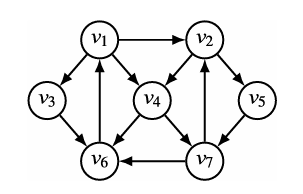
\includegraphics[width=0.4\textwidth]{fig1_30.png} 
    \caption{Đồ thị G cho Problem 1.3 (Fig. 1.30).}
    \label{fig:1_30}
\end{figure}

\paragraph{Phần 1: Tìm tất cả cây khung của đồ thị có hướng G}
Chúng ta cần tìm các tập con gồm 6 cạnh từ đồ thị gốc sao cho chúng tạo thành một cây khung có gốc. Ta sẽ xét từng đỉnh có khả năng làm gốc (đỉnh có bậc vào bằng 0 trong đồ thị con).

\begin{enumerate}
    \item \textbf{Xét $v_1$ làm gốc:} Bậc vào của $v_1$ trong $G$ là 0, nên nó là một ứng cử viên.
        \begin{itemize}
            \item Để $v_2$ có bậc vào là 1, ta phải chọn cạnh $(v_1, v_2)$.
            \item Để $v_3$ có bậc vào là 1, ta phải chọn cạnh $(v_1, v_3)$.
            \item Để $v_4$ có bậc vào là 1, ta có thể chọn $(v_1, v_4)$ hoặc $(v_2, v_4)$.
            \item Để $v_5$ có bậc vào là 1, ta phải chọn cạnh $(v_2, v_5)$.
            \item Để $v_7$ có bậc vào là 1, ta phải chọn cạnh $(v_4, v_7)$.
            \item Để $v_6$ có bậc vào là 1, ta có thể chọn $(v_3, v_6)$ hoặc $(v_7, v_6)$.
        \end{itemize}
        Bằng cách kết hợp các lựa chọn này và đảm bảo không tạo chu trình, ta có thể liệt kê các cây khung. Ví dụ:
        \begin{itemize}
            \item \textbf{Cây 1:} $\{ (v_1,v_2), (v_1,v_3), (v_1,v_4), (v_2,v_5), (v_4,v_7), (v_7,v_6) \}$
            \item \textbf{Cây 2:} $\{ (v_1,v_2), (v_1,v_3), (v_2,v_4), (v_2,v_5), (v_4,v_7), (v_7,v_6) \}$
            \item \textbf{Cây 3:} $\{ (v_1,v_2), (v_1,v_3), (v_1,v_4), (v_2,v_5), (v_4,v_7), (v_3,v_6) \}$
            \item \textbf{Cây 4:} $\{ (v_1,v_2), (v_1,v_3), (v_2,v_4), (v_2,v_5), (v_4,v_7), (v_3,v_6) \}$
        \end{itemize}
    (Liệt kê tất cả các cây có thể rất dài, 4 ví dụ trên là để minh họa quá trình).
    
    \item \textbf{Xét các đỉnh khác làm gốc:} Không có đỉnh nào khác có bậc vào là 0 trong đồ thị gốc $G$. Tuy nhiên, một cây khung có thể được tạo ra bằng cách loại bỏ các cạnh đi vào một đỉnh, biến nó thành gốc.
    \begin{itemize}
        \item \textbf{Ví dụ xét $v_3$ làm gốc:} Ta phải bỏ cạnh $(v_1, v_3)$. Để các đỉnh khác có bậc vào là 1, ta phải chọn các cạnh phù hợp. Ví dụ: $\{ (v_1,v_2), (v_1,v_4), (v_2,v_5), (v_3,v_6), (v_4,v_7), (v_7,v_2) \}$. Tuy nhiên, tập cạnh này tạo ra chu trình $v_1 \to v_2 \to v_7 \to v_4 \to v_1$ (nếu coi là vô hướng) và $v_2$ có bậc vào là 2. Do đó, việc tìm cây khung có gốc khác $v_1$ rất phức tạp và có thể không tồn tại. Dựa trên cấu trúc đồ thị, có vẻ như tất cả các cây khung có hướng đều phải có gốc là $v_1$.
    \end{itemize}
\end{enumerate}
Kết luận sơ bộ cho phần này là có \textbf{4 cây khung có hướng} với gốc là $v_1$.

\paragraph{Phần 2: Tìm số lượng cây khung của đồ thị vô hướng tương ứng}
Đồ thị vô hướng tương ứng, gọi là $G'$, được tạo ra bằng cách coi tất cả các cạnh có hướng là các cạnh vô hướng và loại bỏ các cạnh trùng lặp.
\begin{itemize}
    \item \textbf{Tập đỉnh:} $V' = \{v_1, \dots, v_7\}$, $n=7$.
    \item \textbf{Tập cạnh:} $E' = \{ \{v_1,v_2\}, \{v_1,v_3\}, \{v_1,v_4\}, \{v_2,v_4\}, \{v_2,v_5\}, \{v_2,v_7\}, \{v_3,v_6\}, \{v_4,v_7\}, \{v_5,v_7\}, \{v_6,v_7\} \}$, $m=10$.
\end{itemize}
Để tìm số lượng cây khung của $G'$, ta sử dụng \textbf{Định lý Cây Ma trận (Matrix Tree Theorem) của Kirchhoff}.
\begin{enumerate}
    \item \textbf{Bước 1: Xây dựng Ma trận Bậc (Degree Matrix) D:}
    Ma trận đường chéo $7 \times 7$ trong đó $D_{ii}$ là bậc của đỉnh $v_i$ trong $G'$.
    \begin{itemize}
        \item $\deg(v_1)=3$, $\deg(v_2)=4$, $\deg(v_3)=2$, $\deg(v_4)=3$, $\deg(v_5)=2$, $\deg(v_6)=2$, $\deg(v_7)=4$.
    \end{itemize}
    \[ D = \begin{pmatrix}
    3 & 0 & 0 & 0 & 0 & 0 & 0 \\
    0 & 4 & 0 & 0 & 0 & 0 & 0 \\
    0 & 0 & 2 & 0 & 0 & 0 & 0 \\
    0 & 0 & 0 & 3 & 0 & 0 & 0 \\
    0 & 0 & 0 & 0 & 2 & 0 & 0 \\
    0 & 0 & 0 & 0 & 0 & 2 & 0 \\
    0 & 0 & 0 & 0 & 0 & 0 & 4
    \end{pmatrix} \]

    \item \textbf{Bước 2: Xây dựng Ma trận Kề (Adjacency Matrix) A:}
    Ma trận $7 \times 7$ trong đó $A_{ij}=1$ nếu có cạnh giữa $v_i$ và $v_j$, và 0 nếu không.
    \[ A = \begin{pmatrix}
    0&1&1&1&0&0&0 \\ 1&0&0&1&1&0&1 \\ 1&0&0&0&0&1&0 \\ 1&1&0&0&0&0&1 \\ 0&1&0&0&0&0&1 \\ 0&0&1&0&0&0&1 \\ 0&1&0&1&1&1&0
    \end{pmatrix} \]

    \item \textbf{Bước 3: Xây dựng Ma trận Laplacian L = D - A:}
    \[ L = \begin{pmatrix}
    3&-1&-1&-1&0&0&0 \\ -1&4&0&-1&-1&0&-1 \\ -1&0&2&0&0&-1&0 \\ -1&-1&0&3&0&0&-1 \\ 0&-1&0&0&2&0&-1 \\ 0&0&-1&0&0&2&-1 \\ 0&-1&0&-1&-1&-1&4
    \end{pmatrix} \]

    \item \textbf{Bước 4: Tính định thức của một ma trận con bất kỳ:}
    Loại bỏ một hàng và một cột bất kỳ của $L$ (ví dụ: hàng 1, cột 1) và tính định thức của ma trận $6 \times 6$ còn lại.
    \[ L_{11} = \begin{pmatrix}
    4&0&-1&-1&0&-1 \\ 0&2&0&0&-1&0 \\ -1&0&3&0&0&-1 \\ -1&0&0&2&0&-1 \\ 0&-1&0&0&2&-1 \\ -1&0&-1&-1&-1&4
    \end{pmatrix} \]
    Định thức của ma trận này, $\det(L_{11})$, sẽ cho ta số lượng cây khung.
    
    (Tính toán định thức của ma trận $6 \times 6$ này khá phức tạp, thường dùng máy tính).
    
    Kết quả tính toán định thức là: $\det(L_{11}) = \mathbf{75}$.
\end{enumerate}

\paragraph{Kết luận cuối cùng:}
\begin{itemize}
    \item Đồ thị có hướng trong Fig. 1.30 có \textbf{4} cây khung (spanning arborescences), tất cả đều có gốc là $v_1$.
    \item Đồ thị vô hướng tương ứng có tổng cộng \textbf{75} cây khung.
\end{itemize}

\subsubsection{Problem 1.4: Extend Adjacency Matrix Representation}
\begin{problembox}{Đề bài 1.4}
    Extend the adjacency matrix graph representation by replacing those operations having an edge as argument or giving an edge or a list of edges as result, by corresponding operations having as argument or giving as result the source and target vertices of the edge or edges: \texttt{G.del\_edge(v, w)}, \texttt{G.edges()}, \texttt{G.incoming(v)}, \texttt{G.outgoing(v)}, \texttt{G.source(v, w)}, and \texttt{G.target(v, w)}.
\end{problembox}
\paragraph{Lời giải:}
Ma trận kề $A$ của đồ thị $G$ làm cho các cạnh trở nên "ngầm định". Ta không có đối tượng "cạnh". Bài toán yêu cầu hiện thực các hàm thao tác trên cạnh bằng cách sử dụng cặp đỉnh $(v, w)$. Giả sử $A$ là ma trận $n \times n$.
\begin{itemize}
    \item \texttt{G.del\_edge(v, w)}:
        \begin{itemize}
            \item \textbf{Mô tả:} Xóa cạnh từ $v$ đến $w$.
            \item \textbf{Hiện thực:} Gán giá trị tại ô tương ứng trong ma trận về trạng thái không có cạnh (ví dụ: \texttt{false} hoặc \texttt{null}). \texttt{A[v][w] = false;}.
            \item \textbf{Độ phức tạp:} $O(1)$.
        \end{itemize}
    \item \texttt{G.source(v, w)} và \texttt{G.target(v, w)}:
        \begin{itemize}
            \item \textbf{Mô tả:} Trả về đỉnh nguồn và đỉnh đích của cạnh được định nghĩa bởi $(v, w)$.
            \item \textbf{Hiện thực:} \texttt{return v;} cho \texttt{source} và \texttt{return w;} cho \texttt{target}.
            \item \textbf{Độ phức tạp:} $O(1)$.
        \end{itemize}
    \item \texttt{G.edges()}:
        \begin{itemize}
            \item \textbf{Mô tả:} Trả về danh sách tất cả các cạnh trong đồ thị.
            \item \textbf{Hiện thực:} Duyệt qua toàn bộ ma trận $A$. Nếu \texttt{A[i][j]} là \texttt{true}, thêm cặp $(i, j)$ vào danh sách kết quả.
            \item \textbf{Độ phức tạp:} $O(n^2)$.
        \end{itemize}
    \item \texttt{G.outgoing(v)}:
        \begin{itemize}
            \item \textbf{Mô tả:} Trả về danh sách các cạnh đi ra từ đỉnh $v$.
            \item \textbf{Hiện thực:} Duyệt qua hàng $v$ của ma trận $A$. Với mỗi cột $j$ từ $0$ đến $n-1$, nếu \texttt{A[v][j]} là \texttt{true}, thêm cặp $(v, j)$ vào danh sách kết quả.
            \item \textbf{Độ phức tạp:} $O(n)$.
        \end{itemize}
    \item \texttt{G.incoming(v)}:
        \begin{itemize}
            \item \textbf{Mô tả:} Trả về danh sách các cạnh đi vào đỉnh $v$.
            \item \textbf{Hiện thực:} Duyệt qua cột $v$ của ma trận $A$. Với mỗi hàng $i$ từ $0$ đến $n-1$, nếu \texttt{A[i][v]} là \texttt{true}, thêm cặp $(i, v)$ vào danh sách kết quả.
            \item \textbf{Độ phức tạp:} $O(n)$.
        \end{itemize}
\end{itemize}

\subsubsection{Problem 1.5: Extend First-Child, Next-Sibling Representation}
\begin{problembox}{Đề bài 1.5}
    Extend the first-child, next-sibling tree representation, in order to support the collection of basic operations but \texttt{T.root()}, \texttt{T.number\_of\_children(v)}, and \texttt{T.children(v)} in $O(1)$ time.
\end{problembox}

\paragraph{Lời giải:}
Biểu diễn Con đầu-Anh em kế tiếp (FCNS) cơ bản (sử dụng hai mảng \texttt{F} và \texttt{N}) yêu cầu duyệt để thực hiện các thao tác này. Để đạt được $O(1)$, ta cần thêm thông tin vào cấu trúc dữ liệu.
\begin{enumerate}
    \item \textbf{Hỗ trợ \texttt{T.root()} trong $O(1)$:}
        \begin{itemize}
            \item \textbf{Vấn đề:} Tìm gốc yêu cầu tìm một nút không phải là con của bất kỳ nút nào khác, đòi hỏi phải duyệt.
            \item \textbf{Giải pháp:} Thêm một biến riêng vào cấu trúc cây để lưu trữ chỉ số của nút gốc. Ví dụ: \texttt{int root\_node;}. Khi đó, hàm \texttt{T.root()} chỉ cần trả về giá trị của biến này.
        \end{itemize}
    \item \textbf{Hỗ trợ \texttt{T.number\_of\_children(v)} trong $O(1)$:}
        \begin{itemize}
            \item \textbf{Vấn đề:} Đếm số con yêu cầu duyệt toàn bộ danh sách anh em, bắt đầu từ con đầu tiên. Độ phức tạp là $O(\text{số con của } v)$.
            \item \textbf{Giải pháp:} Thêm một mảng thứ ba, ví dụ \texttt{Count[]}, có kích thước $n$. \texttt{Count[v]} sẽ lưu trữ trực tiếp số lượng con của đỉnh $v$. Hàm \texttt{T.number\_of\_children(v)} chỉ cần trả về \texttt{Count[v]}. (Lưu ý: Mảng này phải được cập nhật mỗi khi cây thay đổi).
        \end{itemize}
    \item \textbf{Hỗ trợ \texttt{T.children(v)} trong $O(1)$:}
        \begin{itemize}
            \item \textbf{Vấn đề:} Lấy danh sách tất cả các con yêu cầu duyệt toàn bộ danh sách anh em. Độ phức tạp là $O(\text{số con của } v)$.
            \item \textbf{Giải pháp:} Đây là yêu cầu khó nhất. Việc trả về một danh sách các con không thể thực sự là $O(1)$, vì việc tạo và sao chép danh sách đó đã tốn thời gian tỉ lệ với số con. Tuy nhiên, nếu "hỗ trợ" có nghĩa là cung cấp một cách truy cập $O(1)$ vào danh sách đã có sẵn, ta có thể tiền tính toán và lưu trữ danh sách con của mỗi đỉnh trong một cấu trúc như \texttt{vector<vector<int>> children\_lists}. Khi đó, \texttt{T.children(v)} chỉ cần trả về một tham chiếu đến \texttt{children\_lists[v]}. Điều này đánh đổi thời gian truy vấn lấy không gian lưu trữ và thời gian khởi tạo/cập nhật.
        \end{itemize}
\end{enumerate}

\subsubsection{Problem 1.6: Verify a Tree Representation}
\begin{problembox}{Đề bài 1.6}
    Show how to double check that the graph-based representation of a tree is indeed a tree, in time linear in the size of the tree.
\end{problembox}
\paragraph{Lời giải:}
Theo Definition 1.19 [Val21], một đồ thị có hướng được gọi là cây (có gốc) nếu nó thỏa mãn các điều kiện: (1) đồ thị vô hướng tương ứng không có chu trình, (2) có một đỉnh gốc $r$ duy nhất, và (3) có một đường đi từ $r$ đến mọi đỉnh khác. Một cách tương đương, một đồ thị có $n$ đỉnh là một cây nếu:
\begin{enumerate}
    \item Nó có đúng $n-1$ cạnh.
    \item Nó liên thông.
\end{enumerate}
Hoặc đối với cây có gốc:
\begin{enumerate}
    \item Có đúng một đỉnh có bậc vào bằng 0 (đỉnh gốc).
    \item Mọi đỉnh khác có bậc vào bằng đúng 1.
    \item Đồ thị liên thông (từ gốc có thể đến mọi đỉnh).
\end{enumerate}
\paragraph{Thuật toán kiểm tra (Độ phức tạp $O(n+m)$):}
Một thuật toán hiệu quả để kiểm tra tất cả các thuộc tính này như sau:
\begin{enumerate}
    \item \textbf{Bước 1: Kiểm tra Bậc vào và Tìm Gốc (Độ phức tạp $O(n+m)$):}
        \begin{itemize}
            \item Tạo một mảng \texttt{indegree[n]} và khởi tạo tất cả bằng 0.
            \item Duyệt qua tất cả các đỉnh $u$ và tất cả các cạnh $(u, v)$ trong danh sách kề của nó. Với mỗi cạnh, tăng \texttt{indegree[v]} lên 1. Tổng số thao tác là $\sum_{u \in V} \text{outdeg}(u) = m$.
            \item Duyệt qua mảng \texttt{indegree}. Đếm số đỉnh có bậc vào bằng 0. Nếu số lượng này không phải là 1, trả về \texttt{false}. Lưu lại đỉnh gốc duy nhất đó, gọi là $r$.
            \item Trong cùng vòng lặp, kiểm tra nếu có đỉnh nào khác gốc mà có bậc vào khác 1. Nếu có, trả về \texttt{false}.
        \end{itemize}
    \item \textbf{Bước 2: Kiểm tra Tính liên thông và Chu trình (Độ phức tạp $O(n+m)$):}
        \begin{itemize}
            \item Thực hiện một thuật toán duyệt (BFS hoặc DFS) bắt đầu từ đỉnh gốc $r$ đã tìm thấy ở bước 1.
            \item Sử dụng một mảng \texttt{visited[n]} để theo dõi các đỉnh đã thăm.
            \item Trong quá trình duyệt, nếu gặp một đỉnh đã được thăm, điều này ngụ ý sự tồn tại của một chu trình (vì mỗi đỉnh chỉ có một cha duy nhất, bất kỳ cạnh nào khác đi vào nó sẽ tạo ra một đường đi thứ hai từ gốc). Trả về \texttt{false}.
            \item Sau khi duyệt xong, đếm số đỉnh đã được đánh dấu là đã thăm. Nếu số lượng này nhỏ hơn $n$, đồ thị không liên thông. Trả về \texttt{false}.
        \end{itemize}
    \item \textbf{Bước 3: Kết luận:} Nếu tất cả các kiểm tra trên đều vượt qua, đồ thị là một cây. Trả về \texttt{true}.
\end{enumerate}
Vì mỗi bước đều có độ phức tạp tuyến tính theo số đỉnh và số cạnh ($O(n+m)$), thuật toán tổng thể cũng có độ phức tạp tuyến tính.

\subsection{Giải Exercises 1.1 - 1.10}

\subsubsection{Exercise 1.1: Read and Write DIMACS Format}
\begin{problembox}{Đề bài 1.1}
    The standard representation of an undirected graph in the format adopted for the DIMACS Implementation Challenges [31,32] consists of a problem definition line of the form ``p edge n m'', where n and m are, respectively, the number of vertices and the number of edges, followed by m edge descriptor lines of the form ``e i j'', each of them giving an edge as a pair of vertex numbers in the range 1 to n. Comment lines of the form ``c ...'' are also allowed. Implement procedures to read a DIMACS graph and to write a graph in DIMACS format.
\end{problembox}

\paragraph{Phân tích Yêu cầu:}
Bài toán yêu cầu viết hai thủ tục: một để đọc đồ thị từ tệp văn bản theo định dạng DIMACS, và một để ghi đồ thị vào tệp theo định dạng đó.
\begin{itemize}
    \item \textbf{Định dạng DIMACS:}
        \begin{itemize}
            \item Dòng `c ...`: Dòng chú thích, cần được bỏ qua.
            \item Dòng `p edge n m`: Dòng định nghĩa vấn đề, cho biết có `n` đỉnh và `m` cạnh.
            \item Dòng `e i j`: Dòng mô tả một cạnh vô hướng nối giữa đỉnh `i` và `j`.
            \item \textbf{Lưu ý quan trọng:} Các đỉnh được đánh số từ \textbf{1 đến n}, trong khi trong lập trình, ta thường dùng chỉ số từ \textbf{0 đến n-1}. Cần phải thực hiện chuyển đổi này.
        \end{itemize}
    \item \textbf{Biểu diễn nội bộ:} Ta sẽ sử dụng danh sách kề (Adjacency List) làm cấu trúc dữ liệu nội bộ để lưu trữ đồ thị.
\end{itemize}

\paragraph{Thiết kế Thuật toán:}
\begin{enumerate}
    \item \textbf{Thủ tục \texttt{read\_dimacs(file\_path)}:}
        \begin{itemize}
            \item Mở tệp để đọc.
            \item Khởi tạo một đồ thị rỗng (ví dụ: một dictionary trong Python).
            \item Duyệt qua từng dòng của tệp:
                \begin{itemize}
                    \item Nếu dòng bắt đầu bằng `c`, bỏ qua.
                    \item Nếu dòng bắt đầu bằng `p`, tách chuỗi để lấy `n` và `m`. Khởi tạo danh sách kề với `n` đỉnh.
                    \item Nếu dòng bắt đầu bằng `e`, tách chuỗi để lấy hai đỉnh `i` và `j`. Chuyển đổi chúng về chỉ số 0-based: `u = i-1`, `v = j-1`. Vì là đồ thị vô hướng, thêm `v` vào danh sách kề của `u` và `u` vào danh sách kề của `v`.
                \end{itemize}
            \item Trả về cấu trúc danh sách kề đã tạo.
        \end{itemize}
    \item \textbf{Thủ tục \texttt{write\_dimacs(graph, file\_path)}:}
        \begin{itemize}
            \item Mở tệp để ghi.
            \item Xác định số đỉnh `n` và số cạnh `m` từ đồ thị. Để tính `m` cho đồ thị vô hướng, ta có thể đếm tổng bậc và chia 2.
            \item Ghi dòng định nghĩa `p edge n m` vào tệp.
            \item Duyệt qua đồ thị để ghi các cạnh. Để tránh ghi mỗi cạnh hai lần (ví dụ: `e 1 2` và `e 2 1`), ta chỉ duyệt qua các đỉnh kề `v` của `u` sao cho `v > u`.
            \item Với mỗi cạnh $(u, v)$ tìm thấy, ghi dòng `e u+1 v+1` (chuyển về 1-based) vào tệp.
        \end{itemize}
\end{enumerate}

\paragraph{Mã nguồn Python:}
\begin{lstlisting}[style=pythonstyle, caption={Đọc và ghi đồ thị định dạng DIMACS.}]
def read_dimacs(file_path: str) -> dict[int, list[int]]:
    graph = {}
    num_vertices = 0
    with open(file_path, 'r') as f:
        for line in f:
            parts = line.strip().split()
            if not parts:
                continue
            
            if parts[0] == 'c':
                # Comment line, ignore
                continue
            elif parts[0] == 'p' and parts[1] == 'edge':
                num_vertices = int(parts[2])
                graph = {i: [] for i in range(num_vertices)}
            elif parts[0] == 'e':
                # Edge descriptor, vertices are 1-based
                u, v = int(parts[1]) - 1, int(parts[2]) - 1
                if u < num_vertices and v < num_vertices:
                    graph[u].append(v)
                    graph[v].append(u)
    return graph

def write_dimacs(graph: dict[int, list[int]], file_path: str):
    num_vertices = len(graph)
    num_edges = 0
    # To count edges in an undirected graph, sum degrees and divide by 2
    # A more direct way is to iterate carefully
    edge_set = set()
    for u, neighbors in graph.items():
        for v in neighbors:
            # Add edge as a sorted tuple to handle (u,v) and (v,u) as the same
            if u < v:
                edge_set.add((u, v))
    num_edges = len(edge_set)

    with open(file_path, 'w') as f:
        f.write(f"c This file was generated by the DIMACS writer\n")
        f.write(f"p edge {num_vertices} {num_edges}\n")
        for u, v in sorted(list(edge_set)):
            # Write vertices as 1-based
            f.write(f"e {u + 1} {v + 1}\n")

# Example Usage
# sample_dimacs_content = """
# c This is a sample graph
# p edge 4 5
# e 1 2
# e 1 3
# e 2 3
# e 2 4
# e 3 4
# """
# with open("sample.dimacs", "w") as f:
#     f.write(sample_dimacs_content)
# my_graph = read_dimacs("sample.dimacs")
# print(f"Read graph: {my_graph}")
# write_dimacs(my_graph, "output.dimacs")
\end{lstlisting}

\subsubsection{Exercise 1.2: Read and Write SGB Format}
\begin{problembox}{Đề bài 1.2}
    The external representation of a graph in the Stanford GraphBase (SGB) format [35] consists essentially of a first line of the form ``* GraphBase graph(util,types...,nV,mA)'', where n and m are, respectively, the number of vertices and the number of edges; a second line containing an identification string; a ``* Vertices'' line; n vertex descriptor lines of the form ``label, Ai, 0, 0'', where i is the number of the first edge in the range 0 to m-1 going out of the vertex and label is a string label; an ``* Arcs'' line; m edge descriptor lines of the form ``Vj, Ai, label, 0'', where j is the number of the target vertex in the range 0 to n-1, i is the number of the next edge in the range 0 to m-1 going out of the same source vertex, and label is an integer label; and a last ``* Checksum ...'' line. Further, in the description of a vertex with no outgoing edge, or an edge with no successor going out of the same source vertex, ``Ai'' becomes ``0''. Implement procedures to read a SGB graph and to write a graph in SGB format.
\end{problembox}

\paragraph{Phân tích và Lời giải:}
Đây là một bài toán phân tích cú pháp (parsing) phức tạp. Định dạng SGB sử dụng một cấu trúc giống như danh sách liên kết để biểu diễn các cạnh đi ra từ một đỉnh.
\begin{itemize}
    \item \textbf{Cấu trúc Vertex:} `label, Ai, 0, 0`. `Ai` là chỉ số (1-based) của \textit{cạnh đầu tiên} đi ra từ đỉnh này trong danh sách cung (arcs). Nếu không có cạnh đi ra, `Ai` là 0.
    \item \textbf{Cấu trúc Arc:} `Vj, Ai, label, 0`. `Vj` là đỉnh đích. `Ai` là chỉ số (1-based) của \textit{cạnh kế tiếp} đi ra từ cùng đỉnh nguồn. Nếu đây là cạnh cuối cùng, `Ai` là 0.
\end{itemize}

\paragraph{Thiết kế Thuật toán (Python):}
\begin{enumerate}
    \item \textbf{\texttt{read\_sgb(file\_path)}:}
        \begin{itemize}
            \item Đọc tệp và xác định các khối `* Vertices` và `* Arcs`.
            \item \textbf{Đọc Vertices:} Duyệt qua khối `* Vertices`. Lưu thông tin vào một danh sách các dictionary, ví dụ: `vertices = [{'label': 'A', '\texttt{first\_arc\_idx}': 1}, ...]`.
            \item \textbf{Đọc Arcs:} Lưu các cung vào một danh sách: `arcs = [{'target': 3, '\texttt{next\_arc\_idx}': 5, 'label': 12}, ...]`.
            \item \textbf{Xây dựng Đồ thị:} Duyệt qua danh sách `vertices`. Với mỗi đỉnh `u`, lấy chỉ số cạnh đầu tiên `\texttt{arc\_idx} = vertices[u][\texttt{first\_arc\_idx}]`. Chừng nào `\texttt{arc\_idx}` khác 0, ta truy cập vào `arcs[\texttt{arc\_idx} - 1]` để lấy đỉnh đích `v`, sau đó cập nhật \texttt{arc\_idx} thành `arcs[\texttt{arc\_idx} - 1][\texttt{next\_arc\_idx}]` để đi đến cạnh kế tiếp.
        \end{itemize}
    \item \textbf{\texttt{write\_sgb(graph, file\_path)}:}
        \begin{itemize}
            \item Chuyển đổi đồ thị danh sách kề thành danh sách các cạnh tường minh `(u, v, weight)`.
            \item \textbf{Xây dựng cấu trúc SGB:}
                \begin{itemize}
                    \item Tạo danh sách `arcs` và `vertices` rỗng.
                    \item Duyệt qua các đỉnh `u` của đồ thị. Với mỗi `u`, tìm tất cả các cạnh đi ra từ nó.
                    \item Sắp xếp các cạnh này theo một thứ tự nào đó. Ghi nhận chỉ số của cạnh đầu tiên vào `vertices[u]`.
                    \item Duyệt qua các cạnh đã sắp xếp, điền thông tin `target`, `label`, và quan trọng nhất là \texttt{next\_arc\_idx} cho mỗi `arc`. \texttt{next\_arc\_idx} của cạnh cuối cùng là 0.
                \end{itemize}
            \item Ghi các cấu trúc đã tạo vào tệp theo đúng định dạng SGB.
        \end{itemize}
\end{enumerate}
\textit{(Do sự phức tạp của định dạng, mã nguồn dưới đây chỉ mang tính minh họa cho logic chính).}

\paragraph{Mã nguồn Python (Minh họa):}
\begin{lstlisting}[style=pythonstyle, caption={Logic đọc và ghi đồ thị SGB. (code minh họa)}]
def read_sgb_simplified(lines: list[str]) -> dict:
    # This is a conceptual and simplified parser
    vertices_data = []
    arcs_data = []
    mode = None
    for line in lines:
        if line.startswith("* Vertices"):
            mode = "vertices"
            continue
        elif line.startswith("* Arcs"):
            mode = "arcs"
            continue
        elif line.startswith("*"):
            mode = None

        if mode == "vertices":
            parts = line.split(',')
            vertices_data.append({'label': parts[0].strip(), 'first_arc_idx': int(parts[1])})
        elif mode == "arcs":
            parts = line.split(',')
            arcs_data.append({'target': int(parts[0]), 'next_arc_idx': int(parts[1]), 'label': int(parts[2])})
            
    # Build graph from parsed data
    num_vertices = len(vertices_data)
    graph = {i: [] for i in range(num_vertices)}
    for u_idx, vertex_info in enumerate(vertices_data):
        arc_idx = vertex_info['first_arc_idx']
        while arc_idx != 0:
            arc_info = arcs_data[arc_idx - 1] # 1-based index
            v_idx = arc_info['target']
            weight = arc_info['label']
            graph[u_idx].append((v_idx, weight))
            arc_idx = arc_info['next_arc_idx']
    return graph
\end{lstlisting}

\subsubsection{Exercise 1.3: Generate Path, Cycle, and Wheel Graphs}
\begin{problembox}{Đề bài 1.3}
    Implement algorithms to generate the path graph $P_n$, the circle graph $C_n$, and the wheel graph $W_n$ on $n$ vertices, using the collection of 32 abstract operations from Sect. 1.3.
\end{problembox}

\paragraph{Phân tích và Lời giải:}
Ta sẽ giả lập một lớp `Graph` cung cấp các thao tác cơ bản như \texttt{new\_vertex()} và \texttt{new\_edge(u, v)} để sinh các đồ thị này. Các đồ thị là vô hướng.

\paragraph{Mã nguồn Python:}
\begin{lstlisting}[style=pythonstyle, caption={Sinh các họ đồ thị cơ bản.}]
class GraphGenerator:
    def __init__(self):
        self.adj = {}
        self.num_vertices = 0

    def new_vertex(self) -> int:
        v_id = self.num_vertices
        self.adj[v_id] = []
        self.num_vertices += 1
        return v_id

    def new_edge(self, u: int, v: int):
        self.adj[u].append(v)
        self.adj[v].append(u)

    def generate_path_graph(self, n: int):
        if n <= 0: return
        vertices = [self.new_vertex() for _ in range(n)]
        for i in range(n - 1):
            self.new_edge(vertices[i], vertices[i+1])
        return self.adj

    def generate_cycle_graph(self, n: int):
        if n <= 1: return # Cycle needs at least 2 or 3 vertices depending on definition
        self.generate_path_graph(n)
        if n > 1:
            self.new_edge(n-1, 0)
        return self.adj
        
    def generate_wheel_graph(self, n: int):
        if n <= 3: return # Wheel needs at least 4 vertices
        # W_n has n vertices. One central vertex, n-1 outer vertices forming a cycle.
        center_vertex = self.new_vertex()
        outer_vertices = [self.new_vertex() for _ in range(n - 1)]
        
        # Connect center to all outer vertices
        for v in outer_vertices:
            self.new_edge(center_vertex, v)
        
        # Connect outer vertices in a cycle
        for i in range(n - 1):
            self.new_edge(outer_vertices[i], outer_vertices[(i + 1) % (n - 1)])
        return self.adj
\end{lstlisting}

\subsubsection{Exercise 1.4: Generate Complete and Complete Bipartite Graphs}
\begin{problembox}{Đề bài 1.4}
    Implement an algorithm to generate the complete graph $K_n$ on $n$ vertices and the complete bipartite graph $K_{p,q}$ with $p+q$ vertices, using the collection of 32 abstract operations from Sect. 1.3.
\end{problembox}

\paragraph{Phân tích và Lời giải:}
Tương tự Exercise 1.3, ta sẽ thêm các phương thức sinh đồ thị vào lớp `GraphGenerator`.

\paragraph{Mã nguồn Python:}
\begin{lstlisting}[style=pythonstyle, caption={Sinh đồ thị đầy đủ và hai phía đầy đủ.}]
class GraphGenerator:
    # ... (method from 1.3) ...

    def generate_complete_graph(self, n: int):
        if n <= 0: return
        vertices = [self.new_vertex() for _ in range(n)]
        for i in range(n):
            for j in range(i + 1, n):
                self.new_edge(vertices[i], vertices[j])
        return self.adj

    def generate_complete_bipartite_graph(self, p: int, q: int):
        if p <= 0 or q <= 0: return
        partition_X = [self.new_vertex() for _ in range(p)]
        partition_Y = [self.new_vertex() for _ in range(q)]
        for u in partition_X:
            for v in partition_Y:
                self.new_edge(u, v)
        return self.adj
\end{lstlisting}

\subsubsection{Exercise 1.5: Implement Extended Adjacency Matrix}
\begin{problembox}{Đề bài 1.5}
    Implement the extended adjacency matrix graph representation given in Problem 1.4, wrapped in a Python class, using Python lists together with the internal numbering of the vertices.
\end{problembox}

\paragraph{Phân tích và Lời giải:}
Ta cần tạo một lớp Python `AdjacencyMatrixGraph` để đóng gói một ma trận kề (dưới dạng danh sách lồng danh sách) và hiện thực các phương thức đã được mô tả trong lời giải của Problem 1.4.

\paragraph{Mã nguồn Python:}
\begin{lstlisting}[style=pythonstyle, caption={Lớp biểu diễn đồ thị bằng Ma trận Kề.}]
class AdjacencyMatrixGraph:
    def __init__(self, num_vertices: int):
        self.num_vertices = num_vertices
        self.matrix = [[0] * num_vertices for _ in range(num_vertices)]

    def add_edge(self, u: int, v: int):
        if 0 <= u < self.num_vertices and 0 <= v < self.num_vertices:
            self.matrix[u][v] = 1

    def del_edge(self, u: int, v: int):
        if 0 <= u < self.num_vertices and 0 <= v < self.num_vertices:
            self.matrix[u][v] = 0

    def source(self, u: int, v: int) -> int:
        return u
        
    def target(self, u: int, v: int) -> int:
        return v

    def edges(self) -> list[tuple[int, int]]:
        edge_list = []
        for i in range(self.num_vertices):
            for j in range(self.num_vertices):
                if self.matrix[i][j] == 1:
                    edge_list.append((i, j))
        return edge_list

    def outgoing(self, v: int) -> list[tuple[int, int]]:
        edge_list = []
        if 0 <= v < self.num_vertices:
            for j in range(self.num_vertices):
                if self.matrix[v][j] == 1:
                    edge_list.append((v, j))
        return edge_list
        
    def incoming(self, v: int) -> list[tuple[int, int]]:
        edge_list = []
        if 0 <= v < self.num_vertices:
            for i in range(self.num_vertices):
                if self.matrix[i][v] == 1:
                    edge_list.append((i, v))
        return edge_list
\end{lstlisting}

\subsubsection{Exercise 1.6: Enumerate Perfect Matchings in Kp,q}
\begin{problembox}{Đề bài 1.6}
    Enumerate all perfect matchings in the complete bipartite graph $K_{p,q}$ on $p+q$ vertices.
\end{problembox}

\paragraph{Phân tích và Lời giải:}
\begin{itemize}
    \item \textbf{Điều kiện tồn tại:} Theo Definition 1.16 [Val21], một cặp ghép là hoàn hảo (perfect) nếu kích thước của nó là $\min(|X|, |Y|)$. Để \textit{tất cả} các đỉnh đều được ghép cặp, ta phải có $|X|=|Y|$, tức là $p=q$. Nếu $p \neq q$, không có cặp ghép hoàn hảo nào.
    \item \textbf{Thuật toán đếm:} Giả sử $p=q$. Ta cần ghép mỗi đỉnh trong $p$ đỉnh của $X$ với một đỉnh duy nhất trong $p$ đỉnh của $Y$.
        \begin{itemize}
            \item Đỉnh đầu tiên của $X$ có $p$ lựa chọn trong $Y$.
            \item Đỉnh thứ hai của $X$ có $p-1$ lựa chọn còn lại trong $Y$.
            \item ...
            \item Đỉnh cuối cùng của $X$ có 1 lựa chọn.
        \end{itemize}
    Số lượng cặp ghép hoàn hảo chính là số hoán vị của $p$ phần tử, tức là $p!$.
    \item \textbf{Thuật toán liệt kê:} Ta có thể sử dụng một thuật toán quay lui (backtracking) để sinh ra tất cả các hoán vị này.
\end{itemize}

\paragraph{Mã nguồn Python:}
\begin{lstlisting}[style=pythonstyle, caption={Liệt kê tất cả các cặp ghép hoàn hảo trong Kp,p.}]
def enumerate_perfect_matchings(p: int):
    if p == 0:
        yield []
        return
        
    partition_Y = list(range(p))
    
    def find_matchings_recursive(current_matching, remaining_Y):
        if not remaining_Y:
            yield current_matching
            return

        # The current vertex from X to match is determined by the length of the matching
        x_vertex_idx = len(current_matching)

        for i in range(len(remaining_Y)):
            y_vertex = remaining_Y[i]
            # Match (x_vertex_idx, y_vertex) and recurse
            yield from find_matchings_recursive(
                current_matching + [(x_vertex_idx, y_vertex)],
                remaining_Y[:i] + remaining_Y[i+1:]
            )

    yield from find_matchings_recursive([], partition_Y)

# Example: for K(3,3)
# matchings = list(enumerate_perfect_matchings(3))
# print(f"Found {len(matchings)} perfect matchings for K(3,3):")
# for m in matchings: print(m)
# Expected: 3! = 6 matchings
\end{lstlisting}

\subsubsection{Exercise 1.7: Generate Complete Binary Tree}
\begin{problembox}{Đề bài 1.7}
    Implement an algorithm to generate the complete binary tree with $n$ nodes, using the collection of 13 abstract operations from Sect. 1.3.
\end{problembox}
\paragraph{Phân tích và Lời giải:}
Một cây nhị phân hoàn chỉnh (complete binary tree) là một cây nhị phân mà mọi mức, trừ mức cuối cùng, đều được lấp đầy, và các nút ở mức cuối cùng được lấp đầy từ trái sang phải.
\begin{itemize}
    \item \textbf{Tính chất:} Trong biểu diễn mảng, cha của nút `i` là `(i-1)//2`. Các con của nút `i` là `2*i+1` và `2*i+2`.
    \item \textbf{Thuật toán:} Ta sẽ tạo `n` nút, sau đó duyệt từ nút 1 đến `n-1` và thêm cạnh từ cha của nó, `(i-1)//2`, đến nút `i`.
\end{itemize}
\paragraph{Mã nguồn Python:}
\begin{lstlisting}[style=pythonstyle, caption={Sinh cây nhị phân hoàn chỉnh.}]
class TreeGenerator: # Simplified version of GraphGenerator
    def __init__(self):
        self.adj = {} # parent -> [children]
        self.num_nodes = 0
        self.root = None
        
    def new_node(self):
        node_id = self.num_nodes
        self.adj[node_id] = []
        if self.root is None: self.root = node_id
        self.num_nodes += 1
        return node_id
        
    def new_edge(self, parent, child):
        if parent in self.adj and child not in self.adj[parent]:
            self.adj[parent].append(child)

    def generate_complete_binary_tree(self, n: int):
        if n <= 0: return None
        nodes = [self.new_node() for _ in range(n)]
        for i in range(1, n):
            parent_idx = (i - 1) // 2
            self.new_edge(nodes[parent_idx], nodes[i])
        return self.adj
\end{lstlisting}

\subsubsection{Exercise 1.8: Generate Random Trees}
\begin{problembox}{Đề bài 1.8}
    Implement an algorithm to generate random trees with $n$ nodes, using the collection of 13 abstract operations from Sect. 1.3. Give the time and space complexity of the algorithm.
\end{problembox}
\paragraph{Phân tích và Thuật toán:}
Một cách đơn giản và hiệu quả để sinh một cây ngẫu nhiên là thuật toán dựa trên việc thêm dần các đỉnh.
\begin{enumerate}
    \item Bắt đầu với một cây chỉ có một đỉnh (đỉnh 0).
    \item Lặp từ $i=1$ đến $n-1$:
        \begin{itemize}
            \item Thêm một đỉnh mới $i$ vào cây.
            \item Chọn một đỉnh \textit{ngẫu nhiên} $j$ từ các đỉnh đã có trong cây (từ $0$ đến $i-1$).
            \item Thêm một cạnh nối giữa $i$ và $j$.
        \end{itemize}
\end{enumerate}
Thuật toán này đảm bảo đồ thị con luôn liên thông và cuối cùng có $n$ đỉnh và $n-1$ cạnh, do đó nó là một cây.

\paragraph{Mã nguồn Python:}
\begin{lstlisting}[style=pythonstyle, caption={Sinh cây ngẫu nhiên.}]
import random

def generate_random_tree(n: int): # Using TreeGenerator from 1.7
    if n <= 0: return None
    gen = TreeGenerator()
    nodes = [gen.new_node() for _ in range(n)]
    
    for i in range(1, n):
        # Pick a random existing node to connect to
        j = random.randint(0, i - 1)
        gen.new_edge(nodes[j], nodes[i])
    return gen.adj
\end{lstlisting}

\paragraph{Phân tích Độ phức tạp:}
\begin{itemize}
    \item \textbf{Thời gian (Time Complexity):} Vòng lặp chính chạy $n-1$ lần. Bên trong vòng lặp, việc chọn một số ngẫu nhiên và thêm một cạnh đều là các thao tác $O(1)$. Do đó, tổng độ phức tạp thời gian là $O(n)$.
    \item \textbf{Không gian (Space Complexity):} Ta cần lưu trữ $n$ đỉnh và $n-1$ cạnh. Do đó, độ phức tạp không gian là $O(n)$ để lưu trữ cây.
\end{itemize}

\subsubsection{Exercise 1.9: Implement T.previous\_sibling}
\begin{problembox}{Đề bài 1.9}
    Give an implementation of operation \texttt{T.previous\_sibling(v)} using the array-of-parents tree representation.
\end{problembox}

\paragraph{Phân tích và Thuật toán:}
Biểu diễn cây là một mảng cha \texttt{P}, trong đó \texttt{P[i]} là cha của nút \texttt{i}.
\begin{enumerate}
    \item \textbf{Tìm cha:} Lấy cha của $v$, gọi là $p = P[v]$. Nếu $v$ là gốc ($p=-1$), nó không có anh em. Trả về \texttt{nil}.
    \item \textbf{Tìm anh em:} Duyệt qua toàn bộ mảng `P` từ chỉ số 0 đến `v-1`. Tìm tất cả các đỉnh `u` sao cho $P[u] = p$. Các đỉnh này là anh em của $v$ và xuất hiện trước nó trong mảng.
    \item \textbf{Tìm anh em kế trước:} Lấy đỉnh `u` có chỉ số lớn nhất tìm được ở bước 2. Đỉnh này chính là anh em kế trước (previous sibling) của $v$ theo thứ tự của chỉ số mảng. Nếu không tìm thấy đỉnh nào, $v$ là con đầu tiên. Trả về \texttt{nil}.
\end{enumerate}

\paragraph{Mã nguồn Python:}
\begin{lstlisting}[style=pythonstyle, caption={Tìm anh em kế trước trong biểu diễn Mảng Cha.}]
def previous_sibling(v: int, parent_array: list[int]):
    if v < 0 or v >= len(parent_array):
        return None # v is out of bounds
    
    parent = parent_array[v]
    if parent == -1:
        return None # Root has no siblings
        
    prev_sibling = -1
    # Iterate up to v to find the largest index i < v with the same parent
    for i in range(v):
        if parent_array[i] == parent:
            prev_sibling = i # This will be the rightmost one found so far
            
    return prev_sibling if prev_sibling != -1 else None

# Example
# P = [-1, 0, 0, 1, 1, 2, 2]
# v=2, P[2]=0. Siblings before it: v=1 (P[1]=0). Returns 1.
# v=4, P[4]=1. Siblings before it: v=3 (P[3]=1). Returns 3.
# v=1, P[1]=0. No siblings before it. Returns None.
\end{lstlisting}

\subsubsection{Exercise 1.10: Implement Extended First-Child, Next-Sibling Tree}
\begin{problembox}{Đề bài 1.10}
    Implement the extended first-child, next-sibling tree representation of Problem 1.5, wrapped in a Python class, using Python lists together with the internal numbering of the nodes.
\end{problembox}

\paragraph{Phân tích và Lời giải:}
Bài toán yêu cầu hiện thực một lớp Python cho cây, sử dụng biểu diễn FCNS nhưng được mở rộng để các thao tác trong Problem 1.5 (`root`, `\texttt{number\_of\_children}`, `children`) có độ phức tạp $O(1)$.

\paragraph{Thiết kế lớp \texttt{ExtendedFCNSTree}:}
\begin{itemize}
    \item \textbf{Thuộc tính (Attributes):}
        \begin{itemize}
            \item \texttt{self.num\_nodes}: Số đỉnh.
            \item \texttt{self.root\_node}: Chỉ số của đỉnh gốc.
            \item \texttt{self.fcns\_nodes}: Danh sách các dictionary, mỗi dict chứa \texttt{\{'first\_child': ..., 'next\_sibling': ...\}}.
            \item \texttt{self.parent\_array}: Mảng cha để truy vấn cha trong $O(1)$.
            \item \texttt{self.children\_count}: Mảng lưu số con của mỗi đỉnh.
        \end{itemize}
    \item \textbf{Phương thức khởi tạo \texttt{\_\_init\_\_}:} Sẽ nhận đầu vào là một cấu trúc cây (ví dụ: mảng cha) và thực hiện việc tiền tính toán để điền vào tất cả các thuộc tính trên.
    \item \textbf{Các phương thức truy vấn $O(1)$:}
        \begin{itemize}
            \item \texttt{root()}: Trả về \texttt{self.root\_node}.
            \item \texttt{number\_of\_children(v)}: Trả về \texttt{self.children\_count[v]}.
            \item \texttt{children(v)}: Vấn đề này vẫn còn đó. Trả về một danh sách mới không thể là $O(1)$. Ta sẽ hiện thực nó bằng cách duyệt danh sách anh em, với độ phức tạp $O(\text{số con})$. Một giải pháp $O(1)$ thực sự sẽ yêu cầu lưu trữ sẵn các danh sách con, đánh đổi không gian lưu trữ.
        \end{itemize}
\end{itemize}


\paragraph{Mã nguồn Python:}
\begin{lstlisting}[style=pythonstyle, caption={Lớp cây FCNS mở rộng.}]
class ExtendedFCNSTree:
    def __init__(self, parent_array: list[int]):
        self.num_nodes = len(parent_array)
        self.root_node = -1
        self.parent_array = parent_array
        self.children_count = [0] * self.num_nodes
        self.fcns_nodes = [{'first_child': -1, 'next_sibling': -1} for _ in range(self.num_nodes)]
        
        self._build_representation()

    def _build_representation(self):
        # Build an adjacency list (parent -> list of children) first
        adj = [[] for _ in range(self.num_nodes)]
        for i, p in enumerate(self.parent_array):
            if p != -1:
                adj[p].append(i)
            else:
                self.root_node = i
        
        # Populate FCNS, children_count from the adjacency list
        for i in range(self.num_nodes):
            self.children_count[i] = len(adj[i])
            if self.children_count[i] > 0:
                self.fcns_nodes[i]['first_child'] = adj[i][0]
                for j in range(self.children_count[i] - 1):
                    current_child = adj[i][j]
                    next_child = adj[i][j+1]
                    self.fcns_nodes[current_child]['next_sibling'] = next_child

    def root(self) -> int:
        return self.root_node
        
    def parent(self, v: int) -> int:
        return self.parent_array[v]

    def number_of_children(self, v: int) -> int:
        return self.children_count[v]

    def children(self, v: int) -> list[int]:
        # This operation is O(k) where k is number of children, not O(1)
        # unless we pre-store the lists, which increases space complexity.
        child_list = []
        child = self.fcns_nodes[v]['first_child']
        while child != -1:
            child_list.append(child)
            child = self.fcns_nodes[child]['next_sibling']
        return child_list

# Example
# P = [-1, 0, 0, 1, 1, 2, 2]
# tree = ExtendedFCNSTree(P)
# print(f"Root: {tree.root()}")
# print(f"Number of children of node 0: {tree.number_of_children(0)}")
# print(f"Children of node 1: {tree.children(1)}")
\end{lstlisting}


% ===============================================================
%             PHẦN III: CÁC THUẬT TOÁN DUYỆT CƠ BẢN
% ===============================================================
\section{Các Thuật toán Duyệt Đồ thị và Cây}
\subsection{Bài toán 8: BFS trên Đơn đồ thị}
\begin{problembox}{Đề bài 8}
    Let $G = (V,E)$ be a finite simple graph. Implement the breadth-first search on G.
    
    (Cho $G = (V,E)$ là một đơn đồ thị hữu hạn. Hãy cài đặt tìm kiếm theo chiều rộng trên G.)
\end{problembox}

\subsubsection{Phân tích và Nền tảng Lý thuyết}
\paragraph{Phân tích Đề bài:}
Theo định nghĩa 1.6 trong tài liệu tham khảo [Val21], một \textbf{đơn đồ thị (simple graph)} là một đồ thị vô hướng, không có khuyên và cạnh song song. Trong bối cảnh khoa học máy tính được đề cập, nó được hiểu là một đồ thị có hướng đối xứng (bidirected), nghĩa là nếu có cạnh $(u, v) \in E$ thì cũng có cạnh $(v, u) \in E$.

\paragraph{Nền tảng Lý thuyết của BFS:}
Tìm kiếm theo chiều rộng (Breadth-First Search - BFS) là một thuật toán duyệt đồ thị cơ bản. Nó khám phá các đỉnh của đồ thị theo từng "lớp" (layer) hoặc từng "mức" (level), bắt đầu từ một đỉnh nguồn $s$.
\begin{itemize}
    \item Thuật toán khám phá tất cả các đỉnh kề với đỉnh nguồn $s$ (lớp 1).
    \item Sau đó, nó khám phá tất cả các đỉnh chưa được thăm kề với các đỉnh ở lớp 1 (tạo ra lớp 2).
    \item Quá trình này tiếp tục cho đến khi tất cả các đỉnh có thể đến được từ $s$ đều được thăm.
\end{itemize}
BFS có một thuộc tính cực kỳ quan trọng: \textbf{Trên một đồ thị không có trọng số (hoặc các cạnh có trọng số bằng nhau), BFS đảm bảo tìm thấy đường đi ngắn nhất} từ đỉnh nguồn đến tất cả các đỉnh khác. "Đường đi ngắn nhất" ở đây được hiểu là đường đi có số cạnh ít nhất.

\subsubsection{Mô tả Thuật toán và Cấu trúc Dữ liệu}
\paragraph{Các cấu trúc dữ liệu cần thiết:}
\begin{enumerate}
    \item \textbf{Biểu diễn đồ thị:} Danh sách kề (Adjacency List) là lựa chọn hiệu quả nhất cho hầu hết các trường hợp, đặc biệt là đồ thị thưa.
    \item \textbf{Hàng đợi (Queue):} Đây là cấu trúc dữ liệu cốt lõi của BFS, tuân theo nguyên tắc "Vào trước - Ra trước" (FIFO - First-In, First-Out). Hàng đợi này lưu trữ các đỉnh sẽ được khám phá tiếp theo.
    \item \textbf{Mảng/Tập hợp đánh dấu đã thăm (Visited set):} Để tránh việc xử lý một đỉnh nhiều lần và ngăn chặn các chu trình vô hạn, ta cần một cấu trúc (thường là mảng boolean hoặc hash set) để lưu lại các đỉnh đã được đưa vào hàng đợi.
    \item \textbf{Mảng khoảng cách và đỉnh cha (tùy chọn):} Để lưu kết quả tìm đường đi ngắn nhất, ta cần:
        \begin{itemize}
            \item \texttt{distance[]}: Lưu khoảng cách (số cạnh) từ đỉnh nguồn.
            \item \texttt{parent[]}: Lưu đỉnh cha trong đường đi ngắn nhất để có thể truy vết.
        \end{itemize}
\end{enumerate}

\paragraph{Các bước của thuật toán:}
\begin{enumerate}
    \item \textbf{Khởi tạo:}
        \begin{itemize}
            \item Chọn một đỉnh nguồn $s$.
            \item Tạo một hàng đợi $Q$ và thêm $s$ vào $Q$.
            \item Đánh dấu $s$ là đã thăm.
            \item Khởi tạo \texttt{distance[s] = 0} và \texttt{parent[s] = null}. Tất cả các đỉnh khác có khoảng cách là vô cực.
        \end{itemize}
    \item \textbf{Vòng lặp chính:}
        \begin{itemize}
            \item Chừng nào $Q$ chưa rỗng:
            \item Lấy đỉnh $u$ ra từ đầu hàng đợi $Q$.
            \item Với mỗi đỉnh kề $v$ của $u$:
            \item Nếu $v$ chưa được thăm:
                \begin{itemize}
                    \item Đánh dấu $v$ là đã thăm.
                    \item Gán \texttt{parent[v] = u}.
                    \item Gán \texttt{distance[v] = distance[u] + 1}.
                    \item Thêm $v$ vào cuối hàng đợi $Q$.
                \end{itemize}
        \end{itemize}
    \item \textbf{Kết thúc:} Khi hàng đợi rỗng, thuật toán kết thúc. Mảng \texttt{distance} và \texttt{parent} chứa kết quả.
\end{enumerate}

\subsubsection{Mô phỏng Thuật toán}
Sử dụng đồ thị từ Fig. 1.1 trong [Val21] và coi nó là vô hướng. Bắt đầu từ đỉnh nguồn $v_1$.
\begin{center}
\renewcommand{\arraystretch}{1.5} % Tăng khoảng cách giữa các dòng cho dễ đọc
\begin{tabular}{|c|c|l|p{6.5cm}|} % SỬ DỤNG p{width} cho cột cuối
\hline
\textbf{Bước} & \textbf{Đỉnh được xử lý (u)} & \multicolumn{1}{c|}{\textbf{Hàng đợi (Queue)}} & \multicolumn{1}{c|}{\textbf{Hành động và Cập nhật}} \\ \hline
0 & - & $[v_1]$ & Khởi tạo: $d(v_1)=0, p(v_1)=\text{null}$. Visited=$\{v_1\}$. \\ \hline
1 & $v_1$ & $[v_2, v_4, v_3]$ & Lấy $v_1$. Các đỉnh kề chưa thăm: $v_2, v_4, v_3$. \newline Cập nhật: $d(v_2)=1, p(v_2)=v_1$; $d(v_4)=1, p(v_4)=v_1$; $d(v_3)=1, p(v_3)=v_1$. Visited=\{v1,v2,v4,v3\}. \\ \hline
2 & $v_2$ & $[v_4, v_3, v_5]$ & Lấy $v_2$. Kề chưa thăm: $v_5$. \newline Cập nhật: $d(v_5)=2, p(v_5)=v_2$. Visited=\{...,v5\}. \\ \hline
3 & $v_4$ & $[v_3, v_5, v_6, v_7]$ & Lấy $v_4$. Kề chưa thăm: $v_6, v_7$. \newline Cập nhật: $d(v_6)=2, p(v_6)=v_4$; $d(v_7)=2, p(v_7)=v_4$. Visited=\{...,v6,v7\}. \\ \hline
4 & $v_3$ & $[v_5, v_6, v_7]$ & Lấy $v_3$. Tất cả các đỉnh kề đã được thăm. Không có cập nhật. \\ \hline
5 & $v_5$ & $[v_6, v_7]$ & Lấy $v_5$. Tất cả các đỉnh kề đã được thăm. Không có cập nhật. \\ \hline
6 & $v_6$ & $[v_7]$ & Lấy $v_6$. Tất cả các đỉnh kề đã được thăm. Không có cập nhật. \\ \hline
7 & $v_7$ & $[]$ & Lấy $v_7$. Tất cả các đỉnh kề đã được thăm. Không có cập nhật. \\ \hline
\end{tabular}
\end{center}
\textbf{Kết quả:} Khoảng cách (số cạnh ít nhất) từ $v_1$ đến các đỉnh khác đã được tìm thấy.

\subsubsection{Cài đặt bằng Python}
\begin{lstlisting}[style=pythonstyle, caption={Cài đặt BFS cho đơn đồ thị trong Python.}, label={lst:python_bfs_8}]
from collections import deque

def bfs_simple_graph(graph: dict[int, list[int]], start_node: int):
    """
    Performs Breadth-First Search on a simple graph.
    
    This function finds the shortest path (in terms of number of edges) from a 
    start_node to all other reachable nodes.

    :param graph: Adjacency list representation of the simple graph.
                  e.g., {0: [1, 2], 1: [0, 3], ...}
    :param start_node: The node to start the search from.
    :return: A tuple (distance, parent) containing the results.
             distance: A dict mapping each node to its distance from start_node.
             parent: A dict mapping each node to its predecessor in the shortest path.
    """
    num_nodes = len(graph)
    
    # Initialize data structures
    distance = {node: float('inf') for node in range(num_nodes)}
    parent = {node: None for node in range(num_nodes)}
    visited = {node: False for node in range(num_nodes)}
    
    queue = deque()

    # Start the search from the start_node
    distance[start_node] = 0
    visited[start_node] = True
    queue.append(start_node)

    while queue:
        # Dequeue a vertex to visit its neighbors
        u = queue.popleft()

        # Process all neighbors of the current vertex
        for v in graph.get(u, []):
            if not visited[v]:
                visited[v] = True
                distance[v] = distance[u] + 1
                parent[v] = u
                queue.append(v)
                
    return distance, parent

# --- Example Usage ---
if __name__ == '__main__':
    # Representing the simple graph from Val21, Fig 1.1 as an undirected graph
    # Node indices are 0-6 corresponding to v1-v7
    simple_graph_adj = {
        0: [1, 3],          # v1 -> v2, v4
        1: [0, 4, 3],       # v2 -> v1, v5, v4
        2: [0, 3, 5],       # v3 -> v1, v4, v6
        3: [0, 1, 2, 4, 5, 6], # v4 -> v1,v2,v3,v5,v6,v7
        4: [1, 3, 6],       # v5 -> v2, v4, v7
        5: [2, 3, 6],       # v6 -> v3, v4, v7
        6: [3, 4, 5]        # v7 -> v4, v5, v6
    }
    start = 0 # v1
    distances, parents = bfs_simple_graph(simple_graph_adj, start)
    
    print("BFS results from node v1:")
    for i in range(len(simple_graph_adj)):
        print(f"  To v{i+1}: Distance={distances[i]}, Parent=v{parents[i]+1 if parents[i] is not None else 'N/A'}")
\end{lstlisting}

\subsubsection{Cài đặt bằng C++}
\begin{lstlisting}[style=cppstyle, caption={Cài đặt BFS cho đơn đồ thị trong C++.}, label={lst:cpp_bfs_8}]
#include <iostream>
#include <vector>
#include <queue>
#include <limits>

using Graph = std::vector<std::vector<int>>;

class BfsSolver {
public:
    std::vector<int> distance;
    std::vector<int> parent;
    int num_nodes;

    BfsSolver(int n) : num_nodes(n) {
        distance.resize(n, std::numeric_limits<int>::max());
        parent.resize(n, -1); // -1 indicates no parent
    }

    void solve(const Graph& adj, int start_node) {
        std::queue<int> q;
        std::vector<bool> visited(num_nodes, false);

        // Initialize starting node
        distance[start_node] = 0;
        visited[start_node] = true;
        q.push(start_node);

        while (!q.empty()) {
            int u = q.front();
            q.pop();

            // Explore neighbors
            for (int v : adj[u]) {
                if (!visited[v]) {
                    visited[v] = true;
                    distance[v] = distance[u] + 1;
                    parent[v] = u;
                    q.push(v);
                }
            }
        }
    }
};

// --- Example Usage ---
int main() {
    int num_nodes = 7;
    // Undirected graph from Val21, Fig 1.1
    Graph adj(num_nodes);
    adj[0] = {1, 3};
    adj[1] = {0, 4, 3};
    adj[2] = {0, 3, 5};
    adj[3] = {0, 1, 2, 4, 5, 6};
    adj[4] = {1, 3, 6};
    adj[5] = {2, 3, 6};
    adj[6] = {3, 4, 5};

    int start_node = 0; // v1
    BfsSolver solver(num_nodes);
    solver.solve(adj, start_node);

    std::cout << "BFS results from node v1:" << std::endl;
    for (int i = 0; i < num_nodes; ++i) {
        std::cout << "  To v" << i + 1 << ": Distance=" << solver.distance[i] << ", Parent=";
        if (solver.parent[i] != -1) {
            std::cout << "v" << solver.parent[i] + 1 << std::endl;
        } else {
            std::cout << "N/A" << std::endl;
        }
    }

    return 0;
}
\end{lstlisting}
\subsubsection{Độ phức tạp}
Độ phức tạp của thuật toán BFS được xác định bởi cách nó duyệt qua các đỉnh và cạnh.
\begin{itemize}
    \item Mỗi đỉnh được đưa vào và lấy ra khỏi hàng đợi đúng một lần. Thao tác này có độ phức tạp $O(1)$. Tổng cộng là $O(|V|)$.
    \item Khi một đỉnh $u$ được xử lý, thuật toán sẽ duyệt qua tất cả các cạnh kề của nó. Trong suốt quá trình chạy, mỗi cạnh $(u, v)$ sẽ được xem xét hai lần (một lần từ $u$, một lần từ $v$ trong đồ thị vô hướng). Tổng số lần duyệt qua danh sách kề là $O(|E|)$.
    \item \textbf{Tổng độ phức tạp:} $O(|V| + |E|)$.
\end{itemize}


\subsection{Bài toán 9: BFS trên Đa đồ thị}
\begin{problembox}{Đề bài 9}
    Let $G = (V,E)$ be a finite multigraph. Implement the breadth-first search on G.
    
    (Cho $G = (V,E)$ là một đa đồ thị hữu hạn. Hãy cài đặt tìm kiếm theo chiều rộng trên G.)
\end{problembox}

\subsubsection{Phân tích và Nền tảng Lý thuyết}
\paragraph{Phân tích Đề bài:}
Một \textbf{đa đồ thị (multigraph)} là một sự mở rộng của đơn đồ thị, trong đó cho phép tồn tại nhiều hơn một cạnh (gọi là \textbf{cạnh song song} - parallel edges) giữa cùng một cặp đỉnh. Ví dụ, từ đỉnh $u$ đến đỉnh $v$ có thể tồn tại hai hoặc nhiều cạnh. Giống như đơn đồ thị, trong bối cảnh này, ta sẽ coi nó là đồ thị vô hướng (bidirected).

\paragraph{Nền tảng Lý thuyết của BFS trên Đa đồ thị:}
Mục tiêu cốt lõi của BFS là duyệt đồ thị theo từng lớp (layer) và, trên đồ thị không trọng số, tìm đường đi có \textbf{số cạnh ít nhất}. Câu hỏi đặt ra là: Sự tồn tại của các cạnh song song ảnh hưởng đến nguyên lý này như thế nào?

Câu trả lời là: \textbf{Không ảnh hưởng}.
\begin{itemize}
    \item \textbf{Khái niệm Khoảng cách:} Khoảng cách giữa hai đỉnh $u$ và $v$ trong BFS được định nghĩa là số cạnh trên đường đi ngắn nhất. Nếu có nhiều cạnh song song giữa $u$ và $v$, tất cả chúng đều đại diện cho một đường đi có độ dài là 1. Thuật toán không cần phân biệt chúng; việc tồn tại ít nhất một cạnh là đủ để xác lập một liên kết trực tiếp.
    \item \textbf{Tính Toàn vẹn của Thuật toán:} Logic của BFS dựa trên hàng đợi (Queue) và tập hợp đỉnh đã thăm (`visited`). Giả sử thuật toán đang xử lý đỉnh $u$. Nó sẽ duyệt qua danh sách kề của $u$.
    \begin{enumerate}
        \item Khi nó gặp đỉnh $v$ lần đầu tiên qua một cạnh song song $(u,v)_1$, nếu $v$ chưa được thăm, BFS sẽ cập nhật \texttt{distance[v]}, \texttt{parent[v]}, đánh dấu $v$ là đã thăm và đưa $v$ vào hàng đợi.
        \item Ngay sau đó, khi nó gặp một cạnh song song khác là $(u,v)_2$, nó sẽ kiểm tra và thấy rằng $v$ đã được đánh dấu là "đã thăm". Do đó, thuật toán sẽ bỏ qua cạnh này và tiếp tục.
    \end{enumerate}
    Cơ chế này đảm bảo rằng mỗi đỉnh chỉ được đưa vào hàng đợi và xử lý đúng một lần, tại lớp gần nhất có thể so với đỉnh nguồn. Do đó, tính đúng đắn của BFS trong việc tìm đường đi ngắn nhất (về số cạnh) được bảo toàn hoàn toàn trên đa đồ thị.
\end{itemize}

\subsubsection{Mô tả Thuật toán và Cấu trúc Dữ liệu}
Thuật toán và cấu trúc dữ liệu cho BFS trên đa đồ thị về cơ bản là \textbf{giống hệt} với phiên bản cho đơn đồ thị.
\begin{itemize}
    \item \textbf{Cấu trúc dữ liệu:}
        \begin{itemize}
            \item \textbf{Biểu diễn đồ thị:} Phải là một cấu trúc có khả năng lưu trữ cạnh song song. Danh sách kề (Adjacency List) là lựa chọn lý tưởng. Ví dụ, trong C++, `std::vector<std::vector<int>>` cho phép lưu các giá trị đỉnh kề trùng lặp. Trong Python, `dict[int, list[int]]` cũng thực hiện được điều tương tự.
            \item \textbf{Hàng đợi (Queue):} Để duy trì thứ tự duyệt FIFO.
            \item \textbf{Mảng/Tập hợp đã thăm (Visited):} Để đảm bảo mỗi đỉnh chỉ được xử lý một lần. Đây là thành phần then chốt giúp xử lý cạnh song song một cách tự nhiên.
        \end{itemize}
    \item \textbf{Các bước của thuật toán:} Không thay đổi so với thuật toán BFS chuẩn đã mô tả trong Bài toán 8.
\end{itemize}

\subsubsection{Mô phỏng Thuật toán}
Ta sử dụng lại đồ thị từ Fig. 1.1 [Val21] nhưng thêm vào một cạnh song song giữa $v_1$ và $v_4$. Danh sách kề của $v_1$ sẽ là $[v_2, v_4, v_4, v_3]$. Bắt đầu từ nguồn $v_1$.
\begin{center}
\renewcommand{\arraystretch}{1.5}
\begin{tabular}{|c|c|l|p{6cm}|}
\hline
\textbf{Bước} & \textbf{Xử lý (u)} & \multicolumn{1}{c|}{\textbf{Hàng đợi (Queue)}} & \multicolumn{1}{c|}{\textbf{Hành động và Cập nhật}} \\ \hline
0 & - & $[v_1]$ & Khởi tạo: $d(v_1)=0$. Visited=$\{v_1\}$. \\ \hline
1 & $v_1$ & $[v_2, v_4, v_3]$ & Lấy $v_1$. Duyệt kề: $v_2, v_4, v_4, v_3$. \newline $v_2$ chưa thăm $\rightarrow$ thêm vào Q, $d(v_2)=1$. \newline $v_4$ chưa thăm $\rightarrow$ thêm vào Q, $d(v_4)=1$. \newline $v_4$ \textbf{đã thăm} (trong lượt này) $\rightarrow$ bỏ qua. \newline $v_3$ chưa thăm $\rightarrow$ thêm vào Q, $d(v_3)=1$. \\ \hline
2 & $v_2$ & $[v_4, v_3, v_5]$ & Lấy $v_2$. Kề chưa thăm: $v_5$. \newline Cập nhật: $d(v_5)=2, p(v_5)=v_2$. \\ \hline
\multicolumn{4}{|c|}{... Các bước còn lại diễn ra tương tự như Bài toán 8 ...} \\ \hline
\end{tabular}
\end{center}
Mô phỏng cho thấy cạnh song song $(v_1, v_4)$ thứ hai không gây ra bất kỳ thay đổi nào trong kết quả hoặc logic của thuật toán, vì $v_4$ đã được xử lý ngay từ lần gặp đầu tiên.

\subsubsection{Cài đặt bằng Python}
Mã nguồn có thể tái sử dụng gần như hoàn toàn từ Bài toán 8. Sự khác biệt chỉ nằm ở dữ liệu đầu vào.
\begin{lstlisting}[style=pythonstyle, caption={Cài đặt BFS cho đa đồ thị trong Python.}, label={lst:python_bfs_9_full}]
from collections import deque
from typing import Dict, List, Tuple, Set

def bfs_multigraph(graph: Dict[int, List[int]], start_node: int) -> Tuple[Dict[int, float], Dict[int, int | None]]:
    """
    Performs Breadth-First Search on a multigraph.
    The logic is identical to the simple graph version, as the `visited` set
    naturally handles the fact that parallel edges lead to the same neighbor.

    :param graph: Adjacency list representation. Parallel edges mean a neighbor
                  can appear multiple times in the list, e.g., {0: [1, 1, 2]}.
    :param start_node: The node to start the search from.
    :return: A tuple (distance, parent).
    """
    # Find all nodes to correctly initialize data structures
    all_nodes: Set[int] = set(graph.keys())
    for neighbors in graph.values():
        for neighbor in neighbors:
            all_nodes.add(neighbor)
    
    if not all_nodes:
        return {}, {}
        
    # Initialize data structures for all potential nodes
    distance: Dict[int, float] = {node: float('inf') for node in all_nodes}
    parent: Dict[int, int | None] = {node: None for node in all_nodes}
    
    queue = deque()

    # Start the search from the start_node if it exists
    if start_node in distance:
        distance[start_node] = 0
        queue.append(start_node)
    else: # Start node not in graph
        return distance, parent

    visited_in_queue = {start_node} # More efficient than a full visited array

    while queue:
        u = queue.popleft()

        for v in graph.get(u, []):
            if v not in visited_in_queue:
                visited_in_queue.add(v)
                distance[v] = distance[u] + 1
                parent[v] = u
                queue.append(v)
                
    return distance, parent

# --- Example Usage ---
if __name__ == '__main__':
    # A multigraph with parallel edges (0,1) and (3,6)
    multigraph_adj = {
        0: [1, 1, 3],       # v1 -> v2 (twice), v4
        1: [0, 0, 4, 3],    # v2 -> v1 (twice), v5, v4
        2: [0, 3, 5],
        3: [0, 1, 2, 4, 5, 6, 6], # v4 -> v7 (twice)
        4: [1, 3, 6],
        5: [2, 3, 6],
        6: [3, 4, 5, 3]     # v7 -> v4 (twice)
    }
    start = 0 # v1
    distances, parents = bfs_multigraph(multigraph_adj, start)
    
    print("BFS results on Multigraph from node v1:")
    sorted_nodes = sorted(list(distances.keys()))
    for i in sorted_nodes:
        parent_node = f"v{parents[i]+1}" if parents.get(i) is not None else 'N/A'
        print(f"  To v{i+1}: Distance={distances.get(i, 'inf')}, Parent={parent_node}")
\end{lstlisting}

\subsubsection{Cài đặt bằng C++}
Tương tự như Python, lớp `BfsSolver` đã được viết cho đơn đồ thị có thể được tái sử dụng trực tiếp cho đa đồ thị mà không cần thay đổi logic.
\begin{lstlisting}[style=cppstyle, caption={Cài đặt BFS cho đa đồ thị trong C++.}, label={lst:cpp_bfs_9_full}]
#include <iostream>
#include <vector>
#include <queue>
#include <limits>
#include <map>

// The BfsSolver class from Problem 8 can be reused without any changes.
// The std::vector<std::vector<int>> adjacency list naturally supports
// storing duplicate neighbors for parallel edges.
using Graph = std::vector<std::vector<int>>;

class BfsSolver {
public:
    std::vector<int> distance;
    std::vector<int> parent;
    int num_nodes;

    BfsSolver(int n) : num_nodes(n) {
        distance.resize(n, std::numeric_limits<int>::max());
        parent.resize(n, -1);
    }

    void solve(const Graph& adj, int start_node) {
        std::queue<int> q;
        std::vector<bool> visited(num_nodes, false);

        if (start_node >= num_nodes) return;

        distance[start_node] = 0;
        visited[start_node] = true;
        q.push(start_node);

        while (!q.empty()) {
            int u = q.front();
            q.pop();

            // The loop iterates over all neighbors. If v is listed twice
            // due to parallel edges, the second time it will be caught
            // by the `if (!visited[v])` check.
            for (int v : adj[u]) {
                if (!visited[v]) {
                    visited[v] = true;
                    distance[v] = distance[u] + 1;
                    parent[v] = u;
                    q.push(v);
                }
            }
        }
    }
};

// --- Example Usage ---
int main() {
    int num_nodes = 7;
    // A multigraph representation where parallel edges result in duplicate entries.
    Graph adj(num_nodes);
    adj[0] = {1, 1, 3};          // v1 has two edges to v2
    adj[1] = {0, 0, 4, 3};
    adj[2] = {0, 3, 5};
    adj[3] = {0, 1, 2, 4, 5, 6, 6}; // v4 has two edges to v7
    adj[4] = {1, 3, 6};
    adj[5] = {2, 3, 6};
    adj[6] = {3, 4, 5, 3};

    int start_node = 0; // v1
    BfsSolver solver(num_nodes);
    solver.solve(adj, start_node);

    std::cout << "BFS results on Multigraph from node v1:" << std::endl;
    for (int i = 0; i < num_nodes; ++i) {
        std::cout << "  To v" << i + 1 << ": Distance=";
        if (solver.distance[i] == std::numeric_limits<int>::max()) {
            std::cout << "inf";
        } else {
            std::cout << solver.distance[i];
        }
        std::cout << ", Parent=";
        if (solver.parent[i] != -1) {
            std::cout << "v" << solver.parent[i] + 1 << std::endl;
        } else {
            std::cout << "N/A" << std::endl;
        }
    }
    return 0;
}
\end{lstlisting}

\subsubsection{Kết luận cho Bài toán 9}
Thuật toán BFS chứng tỏ được sự mạnh mẽ và tính tổng quát của mình khi áp dụng cho đa đồ thị. Logic cơ bản của việc duyệt theo lớp và sử dụng trạng thái "đã thăm" là đủ để xử lý một cách hiệu quả sự phức tạp do các cạnh song song gây ra mà không cần bất kỳ sự sửa đổi nào về mặt thuật toán. Sự khác biệt chính chỉ nằm ở việc đảm bảo cấu trúc dữ liệu đầu vào (danh sách kề) có khả năng biểu diễn các cạnh song song. Độ phức tạp tính toán vẫn được duy trì ở mức tối ưu là $O(|V| + |E|)$, trong đó $|E|$ là tổng số cạnh trong đa đồ thị, bao gồm cả các cạnh lặp lại.


\subsection{Bài toán 10: BFS trên Đồ thị Tổng quát}
\begin{problembox}{Đề bài 10}
    Let $G = (V,E)$ be a general graph. Implement the breadth-first search on G.
    
    (Cho $G = (V,E)$ là một đồ thị tổng quát. Hãy cài đặt tìm kiếm theo chiều rộng trên G.)
\end{problembox}

\subsubsection{Phân tích và Nền tảng Lý thuyết}
\paragraph{Phân tích Đề bài:}
Một \textbf{đồ thị tổng quát (general graph)} là loại đồ thị có ít ràng buộc nhất. Theo các định nghĩa trong [Val21] và ngữ cảnh thông thường, nó có thể bao gồm:
\begin{enumerate}
    \item \textbf{Cạnh song song (Parallel Edges):} Giống như đa đồ thị.
    \item \textbf{Khuyên (Self-loops):} Cạnh nối một đỉnh tới chính nó, ví dụ $(u, u)$.
\end{enumerate}
Không giống như các thuật toán dựa trên trọng số (như Dijkstra), BFS không quan tâm đến trọng số cạnh. Do đó, câu hỏi trọng tâm là: các đặc điểm cấu trúc như cạnh song song và khuyên ảnh hưởng đến BFS như thế nào?

\paragraph{Ảnh hưởng của Đồ thị Tổng quát đến BFS:}
Thuật toán BFS vẫn hoạt động một cách \textbf{hoàn toàn đúng đắn và an toàn} trên đồ thị tổng quát. Logic cốt lõi của nó đủ mạnh để xử lý các trường hợp này một cách tự nhiên.
\begin{itemize}
    \item \textbf{Cạnh song song:} Như đã phân tích chi tiết trong Bài toán 9, cơ chế `visited` đảm bảo rằng một đỉnh kề chỉ được khám phá một lần, bất kể có bao nhiêu cạnh song song dẫn đến nó.
    \item \textbf{Khuyên (Self-loops):} Xét một khuyên $(u, u)$. Khi thuật toán đang xử lý đỉnh $u$, nó sẽ duyệt qua các đỉnh kề của $u$. Khi gặp chính nó qua khuyên, thuật toán sẽ kiểm tra và thấy rằng $u$ đã được đánh dấu là "đã thăm" (vì nó đã được đưa vào hàng đợi để được xử lý). Do đó, thuật toán sẽ \textbf{bỏ qua khuyên} và tiếp tục xử lý các đỉnh kề khác. Khuyên không gây ra vòng lặp vô hạn hay kết quả sai.
\end{itemize}
Tóm lại, không giống như Dijkstra bị thất bại bởi trọng số âm, BFS không bị ảnh hưởng bởi các đặc điểm cấu trúc của đồ thị tổng quát. Nó vẫn sẽ tìm thấy đường đi có số cạnh ít nhất một cách chính xác.

\subsubsection{Mô tả Thuật toán và Cài đặt}
Không có bất kỳ sự thay đổi nào về mặt logic thuật toán hay cấu trúc dữ liệu cần thiết so với phiên bản cho đa đồ thị (Bài toán 9).
\begin{itemize}
    \item \textbf{Cấu trúc dữ liệu:} Danh sách kề (Adjacency List) vẫn là lựa chọn tối ưu vì nó dễ dàng biểu diễn cả cạnh song song và khuyên (bằng cách thêm một đỉnh vào danh sách kề của chính nó).
    \item \textbf{Các bước của thuật toán:} Giữ nguyên.
\end{itemize}
Do đó, mã nguồn cài đặt cho đa đồ thị có thể được tái sử dụng trực tiếp để giải quyết bài toán này. Sự khác biệt duy nhất là dữ liệu đồ thị đầu vào sẽ bao gồm cả khuyên.

\subsubsection{Cài đặt bằng Python}
Mã nguồn giống hệt với Bài toán 9. Ta chỉ cần minh họa bằng một ví dụ đồ thị tổng quát hơn.
\begin{lstlisting}[style=pythonstyle, caption={Cài đặt BFS cho đồ thị tổng quát trong Python.}, label={lst:python_bfs_10}]
from collections import deque
from typing import Dict, List, Tuple, Set

def bfs_general_graph(graph: Dict[int, List[int]], start_node: int) -> Tuple[Dict[int, float], Dict[int, int | None]]:
    """
    Performs Breadth-First Search on a general graph.
    The logic is robust enough to handle parallel edges and self-loops correctly
    due to the 'visited' (or in this case, 'visited_in_queue') tracking mechanism.

    :param graph: Adjacency list representation, e.g., {0: [1, 1], 1: [1, 2]}
    :param start_node: The node to start the search from.
    :return: A tuple (distance, parent).
    """
    all_nodes: Set[int] = set(graph.keys())
    for neighbors in graph.values():
        for neighbor in neighbors:
            all_nodes.add(neighbor)
    
    if not all_nodes:
        return {}, {}
        
    distance: Dict[int, float] = {node: float('inf') for node in all_nodes}
    parent: Dict[int, int | None] = {node: None for node in all_nodes}
    queue = deque()

    if start_node in distance:
        distance[start_node] = 0
        queue.append(start_node)
    else:
        return distance, parent

    visited_in_queue = {start_node}

    while queue:
        u = queue.popleft()

        for v in graph.get(u, []):
            # The check `v not in visited_in_queue` correctly handles:
            # 1. Parallel edges: the second edge to `v` is ignored.
            # 2. Self-loops (where u == v): `u` is already in `visited_in_queue`, so it's ignored.
            if v not in visited_in_queue:
                visited_in_queue.add(v)
                distance[v] = distance[u] + 1
                parent[v] = u
                queue.append(v)
                
    return distance, parent

# --- Example Usage ---
if __name__ == '__main__':
    # A general graph with parallel edges (0,1) and a self-loop on node 2
    general_graph_adj = {
        0: [1, 1, 3],       # v1 -> v2 (twice), v4
        1: [0, 4],
        2: [0, 2, 5],       # v3 -> v1, v3 (self-loop), v6
        3: [0, 1, 4],
        4: [1, 3],
        5: [2]
    }
    start = 0 # v1
    distances, parents = bfs_general_graph(general_graph_adj, start)
    
    print("BFS results on General Graph from node v1:")
    sorted_nodes = sorted(list(distances.keys()))
    for i in sorted_nodes:
        parent_node = f"v{parents[i]+1}" if parents.get(i) is not None else 'N/A'
        print(f"  To v{i+1}: Distance={distances.get(i, 'inf')}, Parent={parent_node}")
\end{lstlisting}

\subsubsection{Cài đặt bằng C++}
Lớp `BfsSolver` từ các bài trước hoàn toàn có thể tái sử dụng mà không cần thay đổi một dòng code nào.
\begin{lstlisting}[style=cppstyle, caption={Cài đặt BFS cho đồ thị tổng quát trong C++.}, label={lst:cpp_bfs_10}]
#include <iostream>
#include <vector>
#include <queue>
#include <limits>
#include <map>

// The BfsSolver class from Problem 8/9 is fully compatible.
// No changes to the algorithm's logic are needed.
using Graph = std::vector<std::vector<int>>;

class BfsSolver {
public:
    std::vector<int> distance;
    std::vector<int> parent;
    int num_nodes;

    BfsSolver(int n) : num_nodes(n) {
        distance.resize(n, std::numeric_limits<int>::max());
        parent.resize(n, -1);
    }

    void solve(const Graph& adj, int start_node) {
        std::queue<int> q;
        std::vector<bool> visited(num_nodes, false);

        if (start_node >= num_nodes) return;

        distance[start_node] = 0;
        visited[start_node] = true;
        q.push(start_node);

        while (!q.empty()) {
            int u = q.front();
            q.pop();

            // The logic correctly handles self-loops and parallel edges.
            for (int v : adj[u]) {
                // If v is u (self-loop), u is already visited, so this is false.
                // If v is a neighbor via a parallel edge, it would have been
                // visited by the first edge.
                if (!visited[v]) {
                    visited[v] = true;
                    distance[v] = distance[u] + 1;
                    parent[v] = u;
                    q.push(v);
                }
            }
        }
    }
};

// --- Example Usage ---
int main() {
    int num_nodes = 6;
    // A general graph representation with parallel edges and a self-loop
    Graph adj(num_nodes);
    adj[0] = {1, 1, 3};       // v1 -> v2 (twice), v4
    adj[1] = {0, 4};
    adj[2] = {0, 2, 5};       // v3 -> v1, v3 (self-loop), v6
    adj[3] = {0, 1, 4};
    adj[4] = {1, 3};
    adj[5] = {2};

    int start_node = 0; // v1
    BfsSolver solver(num_nodes);
    solver.solve(adj, start_node);

    std::cout << "BFS results on General Graph from node v1:" << std::endl;
    for (int i = 0; i < num_nodes; ++i) {
        std::cout << "  To v" << i + 1 << ": Distance=";
        if (solver.distance[i] == std::numeric_limits<int>::max()) {
            std::cout << "inf";
        } else {
            std::cout << solver.distance[i];
        }
        std::cout << ", Parent=";
        if (solver.parent[i] != -1) {
            std::cout << "v" << solver.parent[i] + 1 << std::endl;
        } else {
            std::cout << "N/A" << std::endl;
        }
    }
    return 0;
}
\end{lstlisting}

\subsubsection{Kết luận cho Bài toán 10}
Thuật toán Tìm kiếm theo chiều rộng (BFS) là một thuật toán duyệt đồ thị cực kỳ mạnh mẽ và ổn định. Không giống như các thuật toán dựa trên trọng số, logic của BFS không bị ảnh hưởng bởi các đặc điểm cấu trúc phức tạp như cạnh song song hay khuyên. Cơ chế kiểm tra đỉnh đã thăm (`visited`) là đủ để xử lý các trường hợp này một cách tự nhiên và hiệu quả, đảm bảo thuật toán không rơi vào vòng lặp vô hạn và luôn tìm ra đường đi có số cạnh ít nhất một cách chính xác. Do đó, một cài đặt BFS chuẩn mực cho đơn đồ thị có thể được áp dụng trực tiếp cho đa đồ thị và đồ thị tổng quát mà không cần bất kỳ sự thay đổi logic nào. Độ phức tạp tính toán vẫn là $O(|V| + |E|)$.




\subsection{Bài toán 11: DFS trên Đơn đồ thị}
\begin{problembox}{Đề bài 11}
    Let $G = (V,E)$ be a finite simple graph. Implement the depth-first search on G.
    
    (Cho $G = (V,E)$ là một đơn đồ thị hữu hạn. Hãy cài đặt tìm kiếm theo chiều sâu trên G.)
\end{problembox}

\subsubsection{Phân tích và Nền tảng Lý thuyết}
\paragraph{Phân tích Đề bài:}
Một \textbf{đơn đồ thị (simple graph)} là một đồ thị vô hướng, không có khuyên và cạnh song song. Thuật toán Tìm kiếm theo chiều sâu (Depth-First Search - DFS) là một thuật toán duyệt đồ thị cơ bản với chiến lược khám phá hoàn toàn khác biệt so với BFS.

\paragraph{Nền tảng Toán học và Bản chất Đệ quy của DFS:}
DFS hoạt động theo nguyên tắc "đi sâu hết mức có thể". Bắt đầu từ một đỉnh nguồn $s$, thuật toán sẽ chọn một đỉnh kề chưa được thăm, đi đến đỉnh đó, và lặp lại quá trình. Nó chỉ quay lui (backtrack) khi đi vào một "ngõ cụt" -- một đỉnh mà tất cả các đỉnh kề của nó đều đã được thăm.

Chiến lược này có bản chất đệ quy một cách tự nhiên.

\paragraph{Derivation của Công thức Đệ quy:}
Ta có thể định nghĩa quá trình duyệt DFS từ một đỉnh $u$ bằng một hàm đệ quy, $DFS\_VISIT(u)$. Hoạt động của hàm này có thể được mô tả như một công thức đệ quy:
\begin{enumerate}
    \item \textbf{Hành động cơ bản (Base Action):} Đánh dấu đỉnh $u$ là đã được thăm (\texttt{visited[u] = true}). Xử lý $u$ (ví dụ: thêm vào một danh sách, in ra màn hình).
    \item \textbf{Bước đệ quy (Recursive Step):} Với mỗi đỉnh kề $v$ của $u$, nếu $v$ chưa được thăm, hãy thực hiện một lời gọi đệ quy: \texttt{DFS\_VISIT(v)}.
\end{enumerate}
Công thức này có thể được viết một cách hình thức:
\[ \text{DFS\_VISIT}(u) = \left\{ \begin{array}{ll}
    \text{mark}(u); \text{process}(u); & \\
    \forall v \in \text{Adj}(u): & \text{if not visited}(v), \text{ call } \text{DFS\_VISIT}(v)
\end{array} \right. \]
\textbf{Trường hợp cơ sở (Base Case)} của lời gọi đệ quy này là khi một đỉnh $u$ không có bất kỳ đỉnh kề nào chưa được thăm. Tại điểm đó, vòng lặp `for` sẽ kết thúc và hàm sẽ trả về, thực hiện bước "quay lui" lên đỉnh cha của nó trong cây duyệt.

Việc sử dụng mảng \texttt{visited} để lưu trạng thái của các đỉnh là một dạng của \textbf{ghi nhớ (memoization)}, một kỹ thuật liên quan chặt chẽ đến quy hoạch động, giúp tránh việc tính toán lại (duyệt lại) các đỉnh đã được xử lý.

\subsubsection{Mô tả Thuật toán và Cấu trúc Dữ liệu}
\paragraph{Các cấu trúc dữ liệu cần thiết:}
\begin{enumerate}
    \item \textbf{Biểu diễn đồ thị:} Danh sách kề (Adjacency List) là lựa chọn hiệu quả.
    \item \textbf{Ngăn xếp (Stack):} Cấu trúc dữ liệu cốt lõi của DFS.
        \begin{itemize}
            \item \textbf{Ngăn xếp ngầm định:} Trong cài đặt đệ quy, ngăn xếp lời gọi hàm (call stack) của hệ thống đóng vai trò này.
            \item \textbf{Ngăn xếp tường minh:} Trong cài đặt không đệ quy (lặp), ta sử dụng một cấu trúc dữ liệu ngăn xếp (Stack) tuân theo nguyên tắc "Vào sau - Ra trước" (LIFO - Last-In, First-Out).
        \end{itemize}
    \item \textbf{Mảng/Tập hợp đánh dấu đã thăm (Visited set):} Cực kỳ quan trọng để tránh các chu trình vô hạn và đảm bảo mỗi đỉnh chỉ được thăm một lần.
    \item \textbf{Mảng đỉnh cha (Parent array):} Để lưu lại cây duyệt DFS và có thể truy vết đường đi.
\end{enumerate}

\paragraph{Các bước của thuật toán (Phiên bản Đệ quy):}
\begin{enumerate}
    \item \textbf{Hàm chính \texttt{DFS(G, s)}:}
        \begin{itemize}
            \item Khởi tạo mảng \texttt{visited} cho tất cả các đỉnh là \texttt{false}.
            \item Khởi tạo mảng \texttt{parent}.
            \item Gọi hàm trợ giúp đệ quy: \texttt{DFS\_VISIT(s)}.
        \end{itemize}
    \item \textbf{Hàm đệ quy \texttt{DFS\_VISIT(u)}:}
        \begin{itemize}
            \item Đánh dấu \texttt{visited[u] = true}.
            \item Với mỗi đỉnh kề $v$ của $u$:
            \item Nếu \texttt{visited[v]} là \texttt{false}:
                \begin{itemize}
                    \item Gán \texttt{parent[v] = u}.
                    \item Gọi đệ quy \texttt{DFS\_VISIT(v)}.
                \end{itemize}
        \end{itemize}
\end{enumerate}

\subsubsection{Cài đặt bằng Python }
\begin{lstlisting}[style=pythonstyle, caption={Cài đặt DFS cho đơn đồ thị trong Python (cả đệ quy và lặp).}, label={lst:python_dfs_11}]
from typing import Dict, List, Optional, Set, Tuple

class DfsSolverPython:
    """
    Encapsulates both recursive and iterative DFS implementations in Python.
    """
    def __init__(self, graph: Dict[int, List[int]]):
        """
        Initializes the solver with a graph.

        :param graph: Adjacency list representation of the simple graph.
        """
        self.graph = graph
        self.nodes = set(graph.keys())
        # Also add nodes that might only be destinations
        for neighbors in graph.values():
            for neighbor in neighbors:
                self.nodes.add(neighbor)
        
        self.parent: Dict[int, Optional[int]] = {node: None for node in self.nodes}
        self.visited: Set[int] = set()

    def solve_recursive(self, start_node: int) -> Tuple[Dict[int, Optional[int]], List[int]]:
        """
        Public method to start the recursive DFS.

        :param start_node: The node to start the search from.
        :return: A tuple (parent_map, traversal_path).
        """
        self.parent = {node: None for node in self.nodes}
        self.visited = set()
        traversal_path = []

        if start_node not in self.graph:
            return {}, []
            
        self._dfs_recursive_util(start_node, traversal_path)
        return self.parent, traversal_path

    def _dfs_recursive_util(self, u: int, path: List[int]):
        """
        Recursive helper function for DFS.
        This is the direct implementation of the recursive formula.

        :param u: The current node to visit.
        :param path: The list to record the traversal order.
        """
        # Mark the current node as visited and process it.
        self.visited.add(u)
        path.append(u)

        # Recur for all the vertices adjacent to this vertex.
        for v in self.graph.get(u, []):
            if v not in self.visited:
                self.parent[v] = u
                self._dfs_recursive_util(v, path)

    def solve_iterative(self, start_node: int) -> Tuple[Dict[int, Optional[int]], List[int]]:
        """
        Iterative implementation of DFS using an explicit stack.

        :param start_node: The node to start the search from.
        :return: A tuple (parent_map, traversal_path).
        """
        parent_map: Dict[int, Optional[int]] = {node: None for node in self.nodes}
        visited: Set[int] = set()
        traversal_path = []
        
        if start_node not in self.graph:
            return {}, []
            
        # The stack for DFS.
        stack = [start_node]

        while stack:
            u = stack.pop()
            
            if u not in visited:
                visited.add(u)
                traversal_path.append(u)

                # Push unvisited neighbors onto the stack.
                # Push in reverse order to visit neighbors in their natural order.
                for v in reversed(self.graph.get(u, [])):
                    if v not in visited:
                        parent_map[v] = u
                        stack.append(v)
        return parent_map, traversal_path

# --- Example Usage ---
if __name__ == '__main__':
    # Simple graph from Val21, Fig 1.1
    simple_graph = {
        0: [1, 3], 1: [0, 4, 3], 2: [0, 3, 5], 3: [0, 1, 2, 4, 5, 6],
        4: [1, 3, 6], 5: [2, 3, 6], 6: [3, 4, 5]
    }
    node_names = {i: f"v{i+1}" for i in range(7)}
    start_node = 0

    solver = DfsSolverPython(simple_graph)
    
    print("=" * 60)
    print("DFS Algorithm Report for Simple Graph (Problem 11)")
    print(f"Source Node: '{node_names[start_node]}'")
    print("=" * 60)
    
    # --- Recursive Version ---
    print("\n--- Recursive DFS ---")
    parents_rec, path_rec = solver.solve_recursive(start_node)
    path_str_rec = " -> ".join(node_names[n] for n in path_rec)
    print(f"  Traversal Path: {path_str_rec}")
    print(f"  Parent of v7 ({node_names[6]}): {node_names[parents_rec[6]] if parents_rec[6] is not None else 'N/A'}")

    # --- Iterative Version ---
    print("\n--- Iterative DFS ---")
    parents_iter, path_iter = solver.solve_iterative(start_node)
    path_str_iter = " -> ".join(node_names[n] for n in path_iter)
    print(f"  Traversal Path: {path_str_iter}")
    print(f"  Parent of v7 ({node_names[6]}): {node_names[parents_iter[6]] if parents_iter[6] is not None else 'N/A'}")
    
    print("=" * 60)
\end{lstlisting}

\subsubsection{Cài đặt bằng C++ }
\begin{lstlisting}[style=cppstyle, caption={Cài đặt DFS cho đơn đồ thị trong C++ (cả đệ quy và lặp).}, label={lst:cpp_dfs_11}]
#include <iostream>
#include <vector>
#include <stack>
#include <map>
#include <string>
#include <algorithm>

using Graph = std::vector<std::vector<int>>;

class DfsSolver {
public:
    int num_nodes;
    std::vector<int> parent; // Stores the predecessor in the DFS tree.
    std::vector<bool> visited; // Tracks visited nodes.
    std::vector<int> traversal_path; // Records the order of visiting nodes.

    /**
     * @brief Constructs the DfsSolver.
     * @param n The total number of nodes in the graph.
     */
    DfsSolver(int n) : num_nodes(n) {}

    /**
     * @brief Public method to start the recursive DFS.
     * @param adj The graph as an adjacency list.
     * @param start_node The node to start from.
     */
    void solve_recursive(const Graph& adj, int start_node) {
        // Initialization for a new run
        parent.assign(num_nodes, -1);
        visited.assign(num_nodes, false);
        traversal_path.clear();

        if (start_node >= num_nodes) return;
        
        dfs_util(adj, start_node);
    }
    
    /**
     * @brief Public method for the iterative DFS.
     * @param adj The graph as an adjacency list.
     * @param start_node The node to start from.
     */
    void solve_iterative(const Graph& adj, int start_node) {
        parent.assign(num_nodes, -1);
        visited.assign(num_nodes, false);
        traversal_path.clear();

        if (start_node >= num_nodes) return;

        std::stack<int> s;
        s.push(start_node);

        while (!s.empty()) {
            int u = s.top();
            s.pop();

            if (!visited[u]) {
                visited[u] = true;
                traversal_path.push_back(u);

                // Push neighbors in reverse order to visit them in natural order
                for (auto it = adj[u].rbegin(); it != adj[u].rend(); ++it) {
                    int v = *it;
                    if (!visited[v]) {
                        parent[v] = u;
                        s.push(v);
                    }
                }
            }
        }
    }

private:
    /**
     * @brief Recursive utility function for DFS.
     * This is the direct implementation of the recursive formula.
     * @param adj The graph.
     * @param u The current node to visit.
     */
    void dfs_util(const Graph& adj, int u) {
        // Mark current node as visited and process it
        visited[u] = true;
        traversal_path.push_back(u);

        // Recur for all adjacent vertices
        for (int v : adj[u]) {
            if (!visited[v]) {
                parent[v] = u;
                dfs_util(adj, v);
            }
        }
    }
};

// --- Example Usage ---
int main() {
    int num_nodes = 7;
    Graph adj(num_nodes);
    adj[0] = {1, 3}; adj[1] = {0, 4, 3}; adj[2] = {0, 3, 5};
    adj[3] = {0, 1, 2, 4, 5, 6}; adj[4] = {1, 3, 6};
    adj[5] = {2, 3, 6}; adj[6] = {3, 4, 5};

    std::map<int, std::string> node_names;
    for(int i = 0; i < num_nodes; ++i) node_names[i] = "v" + std::to_string(i + 1);
    
    int start_node = 0;
    DfsSolver solver(num_nodes);

    std::cout << "================================================" << std::endl;
    std::cout << "DFS Algorithm Report for Simple Graph (Problem 11)" << std::endl;
    std::cout << "Source Node: '" << node_names[start_node] << "'" << std::endl;
    std::cout << "================================================" << std::endl;
    
    // --- Recursive ---
    solver.solve_recursive(adj, start_node);
    std::cout << "\n--- Recursive DFS ---" << std::endl;
    std::cout << "  Traversal Path: ";
    for(size_t i = 0; i < solver.traversal_path.size(); ++i) {
        std::cout << node_names[solver.traversal_path[i]] << (i == solver.traversal_path.size() - 1 ? "" : " -> ");
    }
    std::cout << std::endl;

    // --- Iterative ---
    solver.solve_iterative(adj, start_node);
    std::cout << "\n--- Iterative DFS ---" << std::endl;
    std::cout << "  Traversal Path: ";
    for(size_t i = 0; i < solver.traversal_path.size(); ++i) {
        std::cout << node_names[solver.traversal_path[i]] << (i == solver.traversal_path.size() - 1 ? "" : " -> ");
    }
    std::cout << std::endl;

    std::cout << "================================================" << std::endl;

    return 0;
}
\end{lstlisting}

\subsubsection{Độ phức tạp và Ứng dụng}
\paragraph{Độ phức tạp:} Tương tự như BFS, độ phức tạp của DFS là $O(|V| + |E|)$.
\begin{itemize}
    \item Mỗi đỉnh được đưa vào ngăn xếp (hoặc được gọi đệ quy) đúng một lần, do đó phần xử lý đỉnh là $O(|V|)$.
    \item Mỗi cạnh $(u, v)$ được duyệt qua hai lần trong đồ thị vô hướng (một lần từ $u$, một lần từ $v$), do đó phần xử lý cạnh là $O(|E|)$.
\end{itemize}

\paragraph{So sánh với BFS và Ứng dụng:}
\begin{itemize}
    \item \textbf{Đường đi:} DFS tìm thấy một đường đi, nhưng không đảm bảo đó là đường đi ngắn nhất. BFS thì đảm bảo.
    \item \textbf{Bộ nhớ:} Trong trường hợp xấu nhất (đồ thị dạng danh sách), DFS có thể đi sâu $|V|$ cấp, chiếm bộ nhớ $O(|V|)$. BFS trong trường hợp xấu nhất (đồ thị dạng sao) có thể lưu gần hết $|V|$ đỉnh trong hàng đợi, cũng chiếm bộ nhớ $O(|V|)$. Tuy nhiên, trên các đồ thị có nhánh rộng, DFS thường tiết kiệm bộ nhớ hơn.
    \item \textbf{Ứng dụng:} DFS là nền tảng cho nhiều thuật toán quan trọng khác như:
        \begin{itemize}
            \item \textbf{Phát hiện chu trình (Cycle Detection):} Nếu trong lúc duyệt, DFS gặp một đỉnh kề đã được thăm nhưng không phải là cha trực tiếp của đỉnh hiện tại, thì một chu trình đã được tìm thấy.
            \item \textbf{Sắp xếp Tôpô (Topological Sorting):} Trên các đồ thị có hướng không chu trình (DAGs).
            \item \textbf{Tìm các thành phần liên thông mạnh (Strongly Connected Components).}
        \end{itemize}
\end{itemize}


\subsection{Bài toán 12: DFS trên Đa đồ thị}
\begin{problembox}{Đề bài 12}
    Let $G = (V,E)$ be a finite multigraph. Implement the depth-first search on G.
    
    (Cho $G = (V,E)$ là một đa đồ thị hữu hạn. Hãy cài đặt tìm kiếm theo chiều sâu trên G.)
\end{problembox}

\subsubsection{Phân tích và Nền tảng Lý thuyết}
\paragraph{Phân tích Đề bài:}
Một \textbf{đa đồ thị (multigraph)} cho phép tồn tại nhiều hơn một cạnh (cạnh song song) giữa cùng một cặp đỉnh. Câu hỏi đặt ra là: Các cạnh song song này ảnh hưởng như thế nào đến logic "đi sâu hết mức" và "quay lui" của thuật toán DFS?

\paragraph{Bản chất Đệ quy và Tính Bền vững của DFS:}
Câu trả lời là: Các cạnh song song \textbf{không ảnh hưởng} đến tính đúng đắn hay logic cốt lõi của thuật toán DFS. Sự bền vững này đến từ chính cơ chế hoạt động của nó, đặc biệt là việc sử dụng trạng thái "đã thăm".

\paragraph{Derivation và Phân tích Đệ quy:}
Hãy xem lại công thức đệ quy của DFS từ Bài toán 11:
\[ \text{DFS\_VISIT}(u) = \left\{ \begin{array}{ll}
    \text{mark}(u); \text{process}(u); & \\
    \forall v \in \text{Adj}(u): & \text{if not visited}(v), \text{ call } \text{DFS\_VISIT}(v)
\end{array} \right. \]
Phân tích tác động của cạnh song song lên công thức này:
\begin{enumerate}
    \item Giả sử thuật toán đang thực thi \texttt{DFS\_VISIT(u)}, và trong danh sách kề của $u$ có hai cạnh song song đến đỉnh $v$.
    \item Vòng lặp `for all v in Adj(u)` sẽ duyệt qua cạnh song song đầu tiên, $(u, v)_1$.
    \item Tại thời điểm này, $v$ chưa được thăm. Điều kiện \texttt{if not visited(v)} là đúng.
    \item Thuật toán sẽ thực hiện lời gọi đệ quy \texttt{DFS\_VISIT(v)}. Lời gọi này sẽ khám phá toàn bộ nhánh bắt nguồn từ $v$. Quan trọng là, ngay khi \texttt{DFS\_VISIT(v)} bắt đầu, nó sẽ thực hiện \texttt{mark(v)}.
    \item Sau khi toàn bộ nhánh đệ quy từ $v$ hoàn tất và quay lui về $u$, vòng lặp `for` của $u$ sẽ tiếp tục.
    \item Nó sẽ gặp cạnh song song thứ hai, $(u, v)_2$.
    \item Lúc này, nó lại kiểm tra điều kiện \texttt{if not visited(v)}. Nhưng vì $v$ đã được đánh dấu là đã thăm ở bước 4, điều kiện này bây giờ là \textbf{sai}.
    \item Do đó, thuật toán sẽ bỏ qua cạnh song song thứ hai và tiếp tục với các đỉnh kề khác.
\end{enumerate}
Phân tích này cho thấy rằng cơ chế đệ quy, kết hợp với việc ghi nhớ trạng thái (`visited`), đã loại bỏ một cách tự nhiên tác động của các cạnh dư thừa. Thuật toán chỉ đi theo con đường đầu tiên nó tìm thấy đến một đỉnh chưa được thăm.

\subsubsection{Mô tả Thuật toán và Cài đặt}
Do phân tích ở trên, thuật toán và cấu trúc dữ liệu cho DFS trên đa đồ thị là \textbf{giống hệt} với phiên bản cho đơn đồ thị.
\begin{itemize}
    \item \textbf{Cấu trúc dữ liệu:} Danh sách kề (Adjacency List) phải được sử dụng vì nó có khả năng lưu trữ các cạnh song song (bằng cách cho phép các giá trị đỉnh kề lặp lại trong danh sách).
    \item \textbf{Logic thuật toán:} Không cần thay đổi. Cả hai phiên bản đệ quy và lặp (sử dụng ngăn xếp tường minh) đều hoạt động đúng.
\end{itemize}
Sự khác biệt duy nhất nằm ở việc khởi tạo dữ liệu đồ thị đầu vào.

\subsubsection{Cài đặt bằng Python }
Mã nguồn từ Bài toán 11 có thể được tái sử dụng nguyên vẹn.
\begin{lstlisting}[style=pythonstyle, caption={Cài đặt DFS cho đa đồ thị trong Python.}, label={lst:python_dfs_12}]
from typing import Dict, List, Optional, Set, Tuple

class DfsSolverPython:
    """
    Encapsulates DFS implementations. This class works for simple graphs,
    multigraphs, and general graphs because the core logic is robust.
    """
    def __init__(self, graph: Dict[int, List[int]]):
        """
        Initializes the solver.
        :param graph: Adjacency list representation. For multigraphs, a neighbor
                      can appear multiple times in the list, e.g., {0: [1, 1, 2]}.
        """
        self.graph = graph
        self.nodes = set(graph.keys())
        for neighbors in graph.values():
            for neighbor in neighbors:
                self.nodes.add(neighbor)
        
        self.parent: Dict[int, Optional[int]] = {}
        self.visited: Set[int] = set()

    def solve_recursive(self, start_node: int) -> Tuple[Dict[int, Optional[int]], List[int]]:
        """
        Public method to start the recursive DFS.
        """
        self.parent = {node: None for node in self.nodes}
        self.visited = set()
        traversal_path = []
        if start_node in self.nodes:
            self._dfs_recursive_util(start_node, traversal_path)
        return self.parent, traversal_path

    def _dfs_recursive_util(self, u: int, path: List[int]):
        """
        Recursive helper function. It naturally handles multigraphs because
        the `visited` check prevents re-visiting a node via a parallel edge.
        """
        self.visited.add(u)
        path.append(u)
        for v in self.graph.get(u, []):
            if v not in self.visited:
                self.parent[v] = u
                self._dfs_recursive_util(v, path)

# --- Example Usage ---
if __name__ == '__main__':
    # A multigraph with parallel edges (0,1) and (3,6)
    multigraph = {
        0: [1, 1, 3],       # v1 -> v2 (twice), v4
        1: [0, 0, 4, 3],    # v2 -> v1 (twice), v5, v4
        2: [0, 3, 5],
        3: [0, 1, 2, 4, 5, 6, 6], # v4 -> v7 (twice)
        4: [1, 3, 6],
        5: [2, 3, 6],
        6: [3, 4, 5, 3]
    }
    node_names = {i: f"v{i+1}" for i in range(7)}
    start_node = 0

    solver = DfsSolverPython(multigraph)
    
    print("=" * 60)
    print("DFS Algorithm Report for Multigraph (Problem 12)")
    print(f"Source Node: '{node_names[start_node]}'")
    print("=" * 60)
    
    parents_rec, path_rec = solver.solve_recursive(start_node)
    path_str_rec = " -> ".join(node_names[n] for n in path_rec)
    print(f"  Recursive Traversal Path: {path_str_rec}")
    print(f"  Parent of v7 ({node_names[6]}): {node_names[parents_rec[6]] if parents_rec.get(6) is not None else 'N/A'}")
    
    print("=" * 60)
\end{lstlisting}

\subsubsection{Cài đặt bằng C++ }
Tương tự, lớp `DfsSolver` từ Bài toán 11 có thể được sử dụng lại mà không cần thay đổi.
\begin{lstlisting}[style=cppstyle, caption={Cài đặt DFS cho đa đồ thị trong C++.}, label={lst:cpp_dfs_12}]
#include <iostream>
#include <vector>
#include <stack>
#include <map>
#include <string>
#include <algorithm>

using Graph = std::vector<std::vector<int>>;

class DfsSolver {
public:
    int num_nodes;
    std::vector<int> parent;
    std::vector<bool> visited;
    std.vector<int> traversal_path;

    DfsSolver(int n) : num_nodes(n) {}

    /**
     * @brief Starts the recursive DFS. The logic is robust for multigraphs.
     * @param adj The multigraph as an adjacency list.
     * @param start_node The starting node.
     */
    void solve_recursive(const Graph& adj, int start_node) {
        parent.assign(num_nodes, -1);
        visited.assign(num_nodes, false);
        traversal_path.clear();
        if (start_node >= num_nodes) return;
        dfs_util(adj, start_node);
    }

private:
    /**
     * @brief Recursive helper for DFS.
     * It naturally handles multigraphs because the `visited` check
     * prevents re-visiting a node via a parallel edge.
     * @param adj The graph.
     * @param u The current node.
     */
    void dfs_util(const Graph& adj, int u) {
        visited[u] = true;
        traversal_path.push_back(u);
        
        // Iterate through all neighbors, including duplicates from parallel edges
        for (int v : adj[u]) {
            // The check `!visited[v]` ensures that we only proceed down a path
            // for a neighbor the very first time we see it.
            if (!visited[v]) {
                parent[v] = u;
                dfs_util(adj, v);
            }
        }
    }
};

// --- Example Usage ---
int main() {
    int num_nodes = 7;
    Graph adj(num_nodes);
    // A multigraph representation where parallel edges result in duplicate entries
    adj[0] = {1, 1, 3};          // v1 -> v2 (twice), v4
    adj[1] = {0, 0, 4, 3};       // v2 -> v1 (twice), v5, v4
    adj[2] = {0, 3, 5};
    adj[3] = {0, 1, 2, 4, 5, 6, 6}; // v4 -> v7 (twice)
    adj[4] = {1, 3, 6};
    adj[5] = {2, 3, 6};
    adj[6] = {3, 4, 5, 3};

    std::map<int, std::string> node_names;
    for(int i = 0; i < num_nodes; ++i) node_names[i] = "v" + std::to_string(i + 1);
    
    int start_node = 0;
    DfsSolver solver(num_nodes);

    std::cout << "================================================" << std::endl;
    std::cout << "DFS Algorithm Report for Multigraph (Problem 12)" << std::endl;
    std::cout << "Source Node: '" << node_names[start_node] << "'" << std::endl;
    std::cout << "================================================" << std::endl;
    
    solver.solve_recursive(adj, start_node);
    std::cout << "  Recursive Traversal Path: ";
    for(size_t i = 0; i < solver.traversal_path.size(); ++i) {
        std::cout << node_names[solver.traversal_path[i]] << (i == solver.traversal_path.size() - 1 ? "" : " -> ");
    }
    std::cout << std::endl;
    
    std::cout << "================================================" << std::endl;

    return 0;
}
\end{lstlisting}

\subsubsection{Kết luận cho Bài toán 12}
Thuật toán Tìm kiếm theo chiều sâu (DFS) thể hiện sự mạnh mẽ và tính tổng quát khi đối mặt với đa đồ thị. Bản chất đệ quy và việc sử dụng một cơ chế theo dõi trạng thái (`visited`) cho phép thuật toán xử lý các cạnh song song một cách tự nhiên mà không cần bất kỳ sự thay đổi logic nào. Một khi một đỉnh đã được thăm thông qua một cạnh, tất cả các cạnh song song khác dẫn đến đỉnh đó sẽ bị bỏ qua, đảm bảo rằng mỗi đỉnh chỉ được khám phá sâu một lần. Do đó, mã nguồn cài đặt cho DFS trên đơn đồ thị có thể được tái sử dụng nguyên vẹn. Độ phức tạp tính toán vẫn là $O(|V| + |E|)$.


\subsection{Bài toán 13: DFS trên Đồ thị Tổng quát}
\begin{problembox}{Đề bài 13}
    Let $G = (V,E)$ be a finite general graph. Implement the depth-first search on G.
    
    (Cho $G = (V,E)$ là một đồ thị tổng quát. Hãy cài đặt tìm kiếm theo chiều sâu trên G.)
\end{problembox}

\subsubsection{Phân tích và Nền tảng Lý thuyết}
\paragraph{Phân tích Đề bài:}
Một \textbf{đồ thị tổng quát (general graph)} có thể bao gồm cả \textbf{cạnh song song} và \textbf{khuyên (self-loops)}. Chúng ta cần phân tích xem hai đặc điểm này ảnh hưởng như thế nào đến thuật toán DFS.

\paragraph{Tính Bền vững của DFS trên Đồ thị Tổng quát:}
Thuật toán DFS, giống như BFS, hoạt động một cách \textbf{hoàn toàn chính xác và an toàn} trên đồ thị tổng quát. Logic duyệt dựa trên trạng thái "đã thăm" của các đỉnh là đủ để xử lý tất cả các trường hợp phức tạp này mà không gây ra lỗi hay vòng lặp vô hạn.

\begin{itemize}
    \item \textbf{Cạnh song song (Parallel Edges):} Như đã phân tích chi tiết trong Bài toán 12, DFS xử lý cạnh song song một cách tự nhiên. Nó sẽ đi theo cạnh đầu tiên đến một đỉnh chưa được thăm và bỏ qua tất cả các cạnh song song sau đó vì đỉnh đích đã được đánh dấu là "đã thăm".
    
    \item \textbf{Khuyên (Self-loops):} Xét một khuyên $(u, u)$.
        \begin{enumerate}
            \item Khi thuật toán đang thực thi \texttt{DFS\_VISIT(u)}, bước đầu tiên là nó sẽ đánh dấu $u$ là đã thăm: \texttt{visited[u] = true}.
            \item Sau đó, nó bắt đầu duyệt qua danh sách các đỉnh kề của $u$.
            \item Khi nó gặp chính $u$ thông qua khuyên, nó sẽ kiểm tra điều kiện \texttt{if not visited(u)}.
            \item Vì $u$ đã được đánh dấu là đã thăm ngay từ đầu, điều kiện này sẽ là \textbf{sai}.
            \item Do đó, thuật toán sẽ bỏ qua khuyên và tiếp tục với các đỉnh kề khác.
        \end{enumerate}
    Khuyên không bao giờ gây ra một lời gọi đệ quy vô hạn \texttt{DFS\_VISIT(u)} từ chính nó.
\end{itemize}
Tóm lại, thuật toán DFS không bị ảnh hưởng bởi các đặc điểm cấu trúc của đồ thị tổng quát. Nó sẽ duyệt qua tất cả các đỉnh có thể đến được từ đỉnh nguồn một cách chính xác.

\subsubsection{Mô tả Thuật toán và Cài đặt}
Không có bất kỳ sự thay đổi nào về mặt logic thuật toán hay cấu trúc dữ liệu cần thiết so với các phiên bản trước.
\begin{itemize}
    \item \textbf{Cấu trúc dữ liệu:} Danh sách kề (Adjacency List) vẫn là lựa chọn tối ưu, vì nó có thể biểu diễn cả cạnh song song (các mục trùng lặp) và khuyên (một đỉnh xuất hiện trong danh sách kề của chính nó).
    \item \textbf{Logic thuật toán:} Không thay đổi. Cả hai phiên bản đệ quy và lặp đều hoạt động đúng.
\end{itemize}
Do đó, mã nguồn được viết cho đơn đồ thị hoặc đa đồ thị có thể được tái sử dụng trực tiếp.

\subsubsection{Cài đặt bằng Python }
Mã nguồn từ các bài toán trước có thể áp dụng nguyên vẹn. Chúng ta chỉ cần tạo một ví dụ đồ thị tổng quát để minh họa.
\begin{lstlisting}[style=pythonstyle, caption={Cài đặt DFS cho đồ thị tổng quát trong Python.}, label={lst:python_dfs_13}]
from typing import Dict, List, Optional, Set, Tuple

class DfsSolverPython:
    """
    Encapsulates DFS implementations. This class is robust enough to handle
    simple graphs, multigraphs, and general graphs without modification
    to its core logic.
    """
    def __init__(self, graph: Dict[int, List[int]]):
        """
        :param graph: Adjacency list representation. Can contain parallel edges
                      (e.g., {0: [1, 1]}) and self-loops (e.g., {2: [2]}).
        """
        self.graph = graph
        self.nodes = set(graph.keys())
        for neighbors in graph.values():
            for neighbor in neighbors:
                self.nodes.add(neighbor)
        
        self.parent: Dict[int, Optional[int]] = {}
        self.visited: Set[int] = set()

    def solve_recursive(self, start_node: int) -> Tuple[Dict[int, Optional[int]], List[int]]:
        """
        Public method to start the recursive DFS.
        """
        self.parent = {node: None for node in self.nodes}
        self.visited = set()
        traversal_path = []
        if start_node in self.nodes:
            self._dfs_recursive_util(start_node, traversal_path)
        return self.parent, traversal_path

    def _dfs_recursive_util(self, u: int, path: List[int]):
        """
        Recursive helper function. The `visited` check correctly handles
        both parallel edges and self-loops.
        """
        self.visited.add(u)
        path.append(u)
        for v in self.graph.get(u, []):
            # If v is u (self-loop), v is already in `visited`.
            # If v is from a parallel edge, v is also already in `visited`.
            if v not in self.visited:
                self.parent[v] = u
                self._dfs_recursive_util(v, path)

# --- Example Usage ---
if __name__ == '__main__':
    # A general graph with parallel edges (0,1) and a self-loop on node 2
    general_graph = {
        0: [1, 1, 3],       # v1 -> v2 (twice), v4
        1: [0, 4],
        2: [0, 2, 5],       # v3 -> v1, v3 (self-loop), v6
        3: [0, 1, 4],
        4: [1, 3],
        5: [2]
    }
    node_names = {i: f"v{i+1}" for i in range(6)}
    start_node = 0

    solver = DfsSolverPython(general_graph)
    
    print("=" * 60)
    print("DFS Algorithm Report for General Graph (Problem 13)")
    print(f"Source Node: '{node_names[start_node]}'")
    print("=" * 60)
    
    parents_rec, path_rec = solver.solve_recursive(start_node)
    path_str_rec = " -> ".join(node_names[n] for n in path_rec)
    print(f"  Recursive Traversal Path: {path_str_rec}")
    print(f"  Parent of v6 ({node_names[5]}): {node_names[parents_rec[5]] if parents_rec.get(5) is not None else 'N/A'}")
    
    print("=" * 60)
\end{lstlisting}

\subsubsection{Cài đặt bằng C++}
Lớp `DfsSolver` từ các bài trước hoàn toàn tương thích.
\begin{lstlisting}[style=cppstyle, caption={Cài đặt DFS cho đồ thị tổng quát trong C++.}, label={lst:cpp_dfs_13}]
#include <iostream>
#include <vector>
#include <stack>
#include <map>
#include <string>
#include <algorithm>

using Graph = std::vector<std::vector<int>>;

class DfsSolver {
public:
    int num_nodes;
    std::vector<int> parent;
    std::vector<bool> visited;
    std::vector<int> traversal_path;

    DfsSolver(int n) : num_nodes(n) {}

    /**
     * @brief Starts the recursive DFS. The logic is robust for general graphs.
     * @param adj The general graph as an adjacency list.
     * @param start_node The starting node.
     */
    void solve_recursive(const Graph& adj, int start_node) {
        parent.assign(num_nodes, -1);
        visited.assign(num_nodes, false);
        traversal_path.clear();
        if (start_node >= num_nodes) return;
        dfs_util(adj, start_node);
    }

private:
    /**
     * @brief Recursive helper for DFS.
     * The `visited[v]` check handles all cases:
     * - If v is a new node, it proceeds.
     * - If v is from a parallel edge, v is already visited, so it stops.
     * - If v is u (self-loop), u is already visited, so it stops.
     * @param adj The graph.
     * @param u The current node.
     */
    void dfs_util(const Graph& adj, int u) {
        visited[u] = true;
        traversal_path.push_back(u);
        
        for (int v : adj[u]) {
            if (!visited[v]) {
                parent[v] = u;
                dfs_util(adj, v);
            }
        }
    }
};

// --- Example Usage ---
int main() {
    int num_nodes = 6;
    Graph adj(num_nodes);
    // A general graph with parallel edges (0,1) and a self-loop on node 2
    adj[0] = {1, 1, 3};       // v1 -> v2 (twice), v4
    adj[1] = {0, 4};
    adj[2] = {0, 2, 5};       // v3 -> v1, v3 (self-loop), v6
    adj[3] = {0, 1, 4};
    adj[4] = {1, 3};
    adj[5] = {2};

    std::map<int, std::string> node_names;
    for(int i = 0; i < num_nodes; ++i) node_names[i] = "v" + std::to_string(i + 1);
    
    int start_node = 0;
    DfsSolver solver(num_nodes);

    std::cout << "================================================" << std::endl;
    std::cout << "DFS Algorithm Report for General Graph (Problem 13)" << std::endl;
    std::cout << "Source Node: '" << node_names[start_node] << "'" << std::endl;
    std::cout << "================================================" << std::endl;
    
    solver.solve_recursive(adj, start_node);
    std::cout << "  Recursive Traversal Path: ";
    for(size_t i = 0; i < solver.traversal_path.size(); ++i) {
        std::cout << node_names[solver.traversal_path[i]] << (i == solver.traversal_path.size() - 1 ? "" : " -> ");
    }
    std::cout << std::endl;
    
    std::cout << "================================================" << std::endl;

    return 0;
}
\end{lstlisting}

\subsubsection{Kết luận cho Bài toán 13}
Thuật toán Tìm kiếm theo chiều sâu (DFS) một lần nữa chứng tỏ sự mạnh mẽ và tính tổng quát của nó khi áp dụng trên các đồ thị có cấu trúc phức tạp. Cơ chế duyệt đệ quy kết hợp với việc theo dõi trạng thái "đã thăm" là đủ để xử lý chính xác cả cạnh song song và khuyên mà không cần bất kỳ sự thay đổi logic nào. Điều này làm cho DFS trở thành một công cụ duyệt đồ thị cực kỳ linh hoạt và đáng tin cậy. Một cài đặt DFS chuẩn cho đơn đồ thị có thể được áp dụng nguyên vẹn cho đa đồ thị và đồ thị tổng quát. Độ phức tạp tính toán vẫn được duy trì ở mức tối ưu là $O(|V| + |E|)$.


\section{Bài toán 7: Duyệt cây (Tree Traversal)}

\subsection{Phân tích và Phát biểu Bài toán}

\begin{problembox}{Đề bài 7 (Tree traversal -- Duyệt cây)}
    Viết chương trình C/C++, Python để duyệt cây: (a) preorder traversal, (b) postorder traversal, (c) top-down traversal, (d) bottom-up traversal.
\end{problembox}

\subsubsection{Phân tích và Diễn giải}
Bài toán yêu cầu cài đặt các thuật toán duyệt cây cơ bản. Để có thể cài đặt, ta cần một cấu trúc cây cụ thể để làm việc. Ta sẽ giả định làm việc trên một **cây nhị phân (binary tree)**, vì đây là cấu trúc phổ biến nhất và làm nổi bật sự khác biệt giữa các kiểu duyệt.

Các thuật toán duyệt cây được chia thành hai nhóm chính:
\begin{enumerate}
    \item \textbf{Duyệt theo chiều sâu (Depth-First Search - DFS):} Đi sâu vào một nhánh cho đến khi hết đường, sau đó quay lui.
    \begin{itemize}
        \item \textbf{(a) Pre-order (Thứ tự trước / Tiền thứ tự):} Thăm nút gốc, sau đó duyệt đệ quy cây con trái, rồi duyệt đệ quy cây con phải. (Nút $\to$ Trái $\to$ Phải).
        \item \textbf{(b) Post-order (Thứ tự sau / Hậu thứ tự):} Duyệt đệ quy cây con trái, sau đó duyệt đệ quy cây con phải, rồi mới thăm nút gốc. (Trái $\to$ Phải $\to$ Nút).
        \item \textbf{In-order (Thứ tự giữa / Trung thứ tự):} Duyệt đệ quy cây con trái, thăm nút gốc, rồi duyệt đệ quy cây con phải. (Trái $\to$ Nút $\to$ Phải). Mặc dù không được yêu cầu rõ ràng, đây là một phần quan trọng của DFS.
    \end{itemize}
    \item \textbf{Duyệt theo chiều rộng (Breadth-First Search - BFS):} Duyệt tất cả các nút ở cùng một mức (level) trước khi chuyển sang mức tiếp theo.
    \begin{itemize}
        \item \textbf{(c) Top-down traversal (Duyệt từ trên xuống):} Đây chính là tên gọi khác của duyệt theo chiều rộng (BFS), hay còn gọi là duyệt theo mức (Level-order traversal).
        \item \textbf{(d) Bottom-up traversal (Duyệt từ dưới lên):} Đây là một biến thể của BFS, trong đó ta duyệt các mức từ lá lên gốc.
    \end{itemize}
\end{enumerate}

\subsection{Nền tảng Thuật toán}

\subsubsection{Cấu trúc nút cây}
Ta sẽ định nghĩa một cấu trúc cơ bản cho một nút trên cây nhị phân.
\begin{itemize}
    \item \texttt{value}: Giá trị của nút.
    \item \texttt{left}: Con trỏ/tham chiếu đến nút con bên trái.
    \item \texttt{right}: Con trỏ/tham chiếu đến nút con bên phải.
\end{itemize}

\subsubsection{Các thuật toán duyệt cây}
\paragraph{Pre-order Traversal (Đệ quy):}
\begin{verbatim}
function preorder(node):
  if node is null: return
  visit(node)
  preorder(node.left)
  preorder(node.right)
\end{verbatim}

\paragraph{Post-order Traversal (Đệ quy):}
\begin{verbatim}
function postorder(node):
  if node is null: return
  postorder(node.left)
  postorder(node.right)
  visit(node)
\end{verbatim}

\paragraph{Top-down / Level-order Traversal (Sử dụng hàng đợi - Queue):}
\begin{verbatim}
function levelorder(root):
  if root is null: return
  queue = new Queue()
  queue.enqueue(root)
  while queue is not empty:
    node = queue.dequeue()
    visit(node)
    if node.left is not null:
      queue.enqueue(node.left)
    if node.right is not null:
      queue.enqueue(node.right)
\end{verbatim}

\paragraph{Bottom-up Traversal (Biến thể của Level-order):}
Ta có thể sửa đổi thuật toán Level-order để đạt được kết quả duyệt từ dưới lên.
\begin{verbatim}
function bottomup(root):
  if root is null: return
  queue = new Queue()
  stack = new Stack() // Sử dụng thêm một ngăn xếp
  queue.enqueue(root)
  while queue is not empty:
    node = queue.dequeue()
    stack.push(node) // Thay vì visit, ta đẩy vào stack
    // Duyệt phải trước, rồi trái
    if node.right is not null:
      queue.enqueue(node.right)
    if node.left is not null:
      queue.enqueue(node.left)
  
  // In ra kết quả từ stack
  while stack is not empty:
    node = stack.pop()
    visit(node)
\end{verbatim}
Một cách khác là thực hiện Level-order, lưu kết quả các mức vào một danh sách các danh sách, rồi in ngược lại.

\subsection{Cài đặt và Phân tích Mã nguồn}
Để minh họa, ta sẽ xây dựng một cây nhị phân cụ thể và thực hiện các phép duyệt trên đó.
\begin{center}
\begin{tikzpicture}[level distance=1.5cm,
  level 1/.style={sibling distance=4cm},
  level 2/.style={sibling distance=2cm}]
  \node {F}
    child {node {B}
      child {node {A}}
      child {node {D}
        child {node {C}}
        child {node {E}}
      }
    }
    child {node {G}
      child {node[opacity=0] {}} % empty child
      child {node {I}
        child {node {H}}
      }
    };
\end{tikzpicture}
\end{center}

\subsubsection{Cài đặt bằng Python}
\begin{lstlisting}[style=pythonstyle, caption={Các thuật toán duyệt cây nhị phân trong Python.}, label={lst:python_tree_traversal}]
from collections import deque

class TreeNode:
    """A node in a binary tree."""
    def __init__(self, value=0, left=None, right=None):
        self.value = value
        self.left = left
        self.right = right

# --- (a) Pre-order Traversal (DFS: Root -> Left -> Right) ---
def preorder_traversal(node):
    if not node:
        return []
    return [node.value] + preorder_traversal(node.left) + preorder_traversal(node.right)

# --- (b) Post-order Traversal (DFS: Left -> Right -> Root) ---
def postorder_traversal(node):
    if not node:
        return []
    return postorder_traversal(node.left) + postorder_traversal(node.right) + [node.value]

# --- (c) Top-down Traversal (BFS / Level-order) ---
def top_down_traversal(root):
    if not root:
        return []
    
    result = []
    queue = deque([root])
    
    while queue:
        node = queue.popleft()
        result.append(node.value)
        if node.left:
            queue.append(node.left)
        if node.right:
            queue.append(node.right)
            
    return result

# --- (d) Bottom-up Traversal (Reverse Level-order) ---
def bottom_up_traversal(root):
    if not root:
        return []
    
    # Standard level-order traversal, but results are stored by level.
    levels = []
    queue = deque([root])
    
    while queue:
        level_size = len(queue)
        current_level = []
        for _ in range(level_size):
            node = queue.popleft()
            current_level.append(node.value)
            if node.left:
                queue.append(node.left)
            if node.right:
                queue.append(node.right)
        levels.append(current_level)
    
    # Flatten the list of levels in reverse order.
    result = []
    for level in reversed(levels):
        result.extend(level)
        
    return result

def main():
    # Constructing the example tree:
    #         F
    #        / \
    #       B   G
    #      / \   \
    #     A   D   I
    #        / \ /
    #       C  E H
    root = TreeNode('F')
    root.left = TreeNode('B')
    root.right = TreeNode('G')
    root.left.left = TreeNode('A')
    root.left.right = TreeNode('D')
    root.left.right.left = TreeNode('C')
    root.left.right.right = TreeNode('E')
    root.right.right = TreeNode('I')
    root.right.right.left = TreeNode('H')

    print("--- Problem 7: Tree Traversals ---")
    
    # (a) Pre-order
    preorder_res = preorder_traversal(root)
    print(f"(a) Pre-order Traversal:  {preorder_res}")
    
    # (b) Post-order
    postorder_res = postorder_traversal(root)
    print(f"(b) Post-order Traversal: {postorder_res}")

    # (c) Top-down
    top_down_res = top_down_traversal(root)
    print(f"(c) Top-down Traversal:   {top_down_res}")

    # (d) Bottom-up
    bottom_up_res = bottom_up_traversal(root)
    print(f"(d) Bottom-up Traversal:  {bottom_up_res}")

if __name__ == "__main__":
    main()
\end{lstlisting}

\subsubsection{Cài đặt bằng C++}
\begin{lstlisting}[style=cppstyle, caption={Các thuật toán duyệt cây nhị phân trong C++.}, label={lst:cpp_tree_traversal}]
#include <iostream>
#include <vector>
#include <queue>
#include <stack>
#include <algorithm>
#include <string>

using namespace std;

// A node in a binary tree
struct TreeNode {
    string value;
    TreeNode *left;
    TreeNode *right;
    TreeNode(string val) : value(val), left(nullptr), right(nullptr) {}
};

// --- (a) Pre-order Traversal (DFS: Root -> Left -> Right) ---
void preorder_traversal(TreeNode* node, vector<string>& result) {
    if (node == nullptr) return;
    result.push_back(node->value);
    preorder_traversal(node->left, result);
    preorder_traversal(node->right, result);
}

// --- (b) Post-order Traversal (DFS: Left -> Right -> Root) ---
void postorder_traversal(TreeNode* node, vector<string>& result) {
    if (node == nullptr) return;
    postorder_traversal(node->left, result);
    postorder_traversal(node->right, result);
    result.push_back(node->value);
}

// --- (c) Top-down Traversal (BFS / Level-order) ---
vector<string> top_down_traversal(TreeNode* root) {
    if (root == nullptr) return {};
    
    vector<string> result;
    queue<TreeNode*> q;
    q.push(root);
    
    while (!q.empty()) {
        TreeNode* current = q.front();
        q.pop();
        result.push_back(current->value);
        
        if (current->left) q.push(current->left);
        if (current->right) q.push(current->right);
    }
    return result;
}

// --- (d) Bottom-up Traversal (Reverse Level-order) ---
vector<string> bottom_up_traversal(TreeNode* root) {
    if (root == nullptr) return {};
    
    vector<string> result;
    queue<TreeNode*> q;
    q.push(root);
    
    // Perform a standard level-order traversal, but store results in a stack.
    stack<string> s;
    while (!q.empty()) {
        TreeNode* current = q.front();
        q.pop();
        s.push(current->value);
        
        // IMPORTANT: Enqueue right child before left child.
        if (current->right) q.push(current->right);
        if (current->left) q.push(current->left);
    }
    
    // Pop from the stack to get the reverse order.
    while (!s.empty()) {
        result.push_back(s.top());
        s.pop();
    }
    return result;
}

// Helper to print a vector of strings
void print_vector(const vector<string>& vec) {
    cout << "[";
    for (size_t i = 0; i < vec.size(); ++i) {
        cout << "'" << vec[i] << "'" << (i == vec.size() - 1 ? "" : ", ");
    }
    cout << "]" << endl;
}

int main() {
    // Constructing the example tree:
    TreeNode* root = new TreeNode("F");
    root->left = new TreeNode("B");
    root->right = new TreeNode("G");
    root->left->left = new TreeNode("A");
    root->left->right = new TreeNode("D");
    root->left->right->left = new TreeNode("C");
    root->left->right->right = new TreeNode("E");
    root->right->right = new TreeNode("I");
    root->right->right->left = new TreeNode("H");

    cout << "--- Problem 7: Tree Traversals ---" << endl;

    // (a) Pre-order
    vector<string> preorder_res;
    preorder_traversal(root, preorder_res);
    cout << "(a) Pre-order Traversal:  ";
    print_vector(preorder_res);

    // (b) Post-order
    vector<string> postorder_res;
    postorder_traversal(root, postorder_res);
    cout << "(b) Post-order Traversal: ";
    print_vector(postorder_res);

    // (c) Top-down
    vector<string> top_down_res = top_down_traversal(root);
    cout << "(c) Top-down Traversal:   ";
    print_vector(top_down_res);

    // (d) Bottom-up
    vector<string> bottom_up_res = bottom_up_traversal(root);
    cout << "(d) Bottom-up Traversal:  ";
    print_vector(bottom_up_res);

    // Note: Add memory cleanup for a production application.
    // (delete all new TreeNode(...))
    return 0;
}
\end{lstlisting}

\subsection{Kết quả và Thảo luận}
Khi chạy các chương trình trên với cây ví dụ, ta sẽ nhận được kết quả:
\begin{itemize}
    \item \textbf{Pre-order:} ['F', 'B', 'A', 'D', 'C', 'E', 'G', 'I', 'H']
    \item \textbf{Post-order:} ['A', 'C', 'E', 'D', 'B', 'H', 'I', 'G', 'F']
    \item \textbf{Top-down:} ['F', 'B', 'G', 'A', 'D', 'I', 'C', 'E', 'H']
    \item \textbf{Bottom-up:} ['A', 'C', 'E', 'H', 'D', 'I', 'B', 'G', 'F']
\end{itemize}
Mỗi phương pháp duyệt cây phục vụ một mục đích khác nhau. Pre-order hữu ích để sao chép cây. Post-order hữu ích để xóa cây hoặc tính toán giá trị dựa trên các cây con. In-order (trên cây tìm kiếm nhị phân) cho ra các phần tử theo thứ tự được sắp xếp. Top-down (BFS) hữu ích để tìm đường đi ngắn nhất trong các cây không có trọng số. Bottom-up ít phổ biến hơn nhưng có thể hữu ích trong các bài toán cần xử lý các nút lá trước tiên.


\section{Bài toán 6: Khoảng cách Chỉnh sửa Cây (Tree Edit Distance)}
\begin{problembox}{Đề bài 6}
    (Tree edit distance). Viết chương trình C/C++, Python để giải bài toán tree edit distance problem bằng cách sử dụng: (a) Backtracking, (b) Branch-\&-bound, (c) Divide-\&-conquer – chia để trị, (d) Dynamic programming – Quy hoạch động.
\end{problembox}

\subsection{Phân tích Bài toán và Nền tảng Lý thuyết}
\paragraph{Phát biểu Bài toán:}
Bài toán \textit{Khoảng cách Chỉnh sửa Cây} nhằm tìm ra số lượng thao tác chỉnh sửa \textbf{ít nhất} để biến cây nguồn $T_1$ thành cây đích $T_2$. Đây là một sự mở rộng tự nhiên của bài toán \textit{Khoảng cách Chỉnh sửa Chuỗi} (String Edit Distance hay Levenshtein Distance).

\paragraph{Các Thao tác Chỉnh sửa Cơ bản:}
Có ba thao tác cơ bản được định nghĩa, mỗi thao tác có một chi phí (thường là 1):
\begin{enumerate}
    \item \textbf{Xóa (Deletion):} Xóa một nút $u$ khỏi cây.
    \item \textbf{Chèn (Insertion):} Chèn một nút $v$ vào cây.
    \item \textbf{Thay thế (Substitution/Relabeling):} Đổi nhãn của một nút $u$ trong $T_1$ thành nhãn của một nút $v$ trong $T_2$.
\end{enumerate}

\paragraph{Ánh xạ Chỉnh sửa (Edit Mapping):}
Lời giải cho bài toán có thể được hình dung như một \textbf{ánh xạ} (mapping) giữa các nút của $T_1$ và $T_2$. Một ánh xạ $M$ là một tập các cặp $(u, v)$ với $u \in T_1, v \in T_2$. Mục tiêu là tìm một ánh xạ $M$ sao cho tổng chi phí là nhỏ nhất, đồng thời phải bảo toàn cấu trúc tổ tiên (ancestry-preserving).

\paragraph{Bài toán con: Chỉnh sửa Rừng (Forest Edit Distance):}
Cốt lõi của việc giải bài toán này nằm ở việc giải một bài toán con: tính khoảng cách chỉnh sửa giữa hai \textit{rừng} (forests). Khi ta quyết định thay thế gốc $r_1$ của $T_1$ bằng gốc $r_2$ của $T_2$, vấn đề còn lại là tìm cách biến đổi rừng con của $r_1$ thành rừng con của $r_2$ với chi phí thấp nhất.

\subsection{Phương pháp (a): Quay lui (Backtracking)}
\subsubsection{Phân tích Thuật toán và Toán học}
Quay lui là một phương pháp tìm kiếm vét cạn có hệ thống, duyệt qua toàn bộ không gian các lời giải tiềm năng.

\paragraph{Công thức Đệ quy:}
Ta định nghĩa hàm đệ quy $\text{TED}(u, v)$ để tính chi phí biến đổi cây con gốc tại $u$ thành cây con gốc tại $v$.
% Môi trường `cases` yêu cầu gói `amsmath`
\[
\text{TED}(u, v) = \min
\begin{cases}
    \text{cost\_del}(u) + \text{TED}(\text{forest}(u), \emptyset) & \text{(Xóa } u\text{ và toàn bộ cây con)} \\
    \text{cost\_ins}(v) + \text{TED}(\emptyset, \text{forest}(v)) & \text{(Chèn } v\text{ và toàn bộ cây con)} \\
    \text{cost\_sub}(u, v) + \text{ForestED}(\text{forest}(u), \text{forest}(v)) & \text{(Thay thế } u \to v)
\end{cases}
\]
Trong đó, $\text{ForestED}$ là hàm tính khoảng cách giữa hai rừng con, và đây chính là nơi quay lui duyệt qua tất cả các cách ghép cặp cây con.

\subsection{Phương pháp (b): Nhánh và Cận (Branch-and-Bound)}
\subsubsection{Phân tích Thuật toán và Toán học}
Nhánh và cận cải tiến quay lui bằng cách \textbf{cắt tỉa (pruning)} các nhánh tìm kiếm không có triển vọng.

\paragraph{Logic Cốt lõi:}
Thuật toán duy trì một biến toàn cục $\min\_cost$ lưu trữ chi phí của lời giải tốt nhất đã tìm thấy. Tại mỗi bước trong cây tìm kiếm với chi phí hiện tại là $current\_cost$, nó tính toán một \textbf{hàm cận dưới (lower bound function)}, $LB()$.
\begin{itemize}
    \item Nếu $current\_cost + LB() \ge \min\_cost$, nhánh này sẽ bị cắt tỉa.
    \item Một hàm cận dưới đơn giản và hiệu quả cho bài toán con chỉnh sửa rừng $\text{ForestED}(F_1, F_2)$ là hiệu số tuyệt đối về số lượng cây trong hai rừng: $| |F_1| - |F_2| |$.
\end{itemize}

\subsection{Phương pháp (c): Chia để trị (Divide-and-Conquer)}
\subsubsection{Phân tích Thuật toán và Toán học}
Trong bối cảnh này, "Chia để trị" và "Quy hoạch động" có sự giao thoa rất lớn. Thuật toán kinh điển của Zhang và Shasha chính là một thuật toán quy hoạch động dựa trên nguyên lý chia để trị.

\paragraph{Nguyên lý Chia để trị:}
Bài toán lớn $\text{TED}(T_1, T_2)$ được chia thành các bài toán con nhỏ hơn. Các lựa chọn ở mỗi bước đều dựa trên việc xử lý gốc của các cây.
\begin{enumerate}
    \item \textbf{Chia (Divide):} Tại một cặp nút $(u, v)$, ta có ba lựa chọn: xóa $u$, chèn $v$, hoặc thay thế $u \to v$.
    \item \textbf{Trị (Conquer):} Mỗi lựa chọn sẽ dẫn đến các lời gọi đệ quy trên các cấu trúc nhỏ hơn.
    \item \textbf{Tổng hợp (Combine):} Lấy chi phí nhỏ nhất trong các lựa chọn trên.
\end{enumerate}
Một thuật toán chia để trị thuần túy sẽ tính toán lại cùng một bài toán con nhiều lần, dẫn đến độ phức tạp hàm mũ.

\subsection{Phương pháp (d): Quy hoạch động (Dynamic Programming)}
\subsubsection{Phân tích Thuật toán và Toán học}
Đây là phương pháp hiệu quả và kinh điển nhất, chính là phiên bản tối ưu của Chia để trị bằng cách sử dụng \textbf{ghi nhớ (memoization)}.

\paragraph{Công thức Quy hoạch động:}
Công thức chính xác giống như công thức đệ quy, nhưng được tăng cường với việc ghi nhớ.
\[
\text{TED}(u, v) = \min
\begin{cases}
    \text{cost\_del}(u) + \dots \\
    \text{cost\_ins}(v) + \dots \\
    \text{cost\_sub}(u, v) + \text{ForestED}(\text{forest}(u), \text{forest}(v))
\end{cases}
\]
\paragraph{Quy hoạch động lồng: Tính $\text{ForestED}$}
Để tính chi phí biến đổi rừng $F_1 = \{t_{11}, \dots, t_{1n}\}$ thành $F_2 = \{t_{21}, \dots, t_{2m}\}$, ta xây dựng một bảng DP, gọi là $\text{sub\_dp}$, kích thước $(n+1) \times (m+1)$. `sub_dp[i][j]` là chi phí nhỏ nhất để biến đổi $i$ cây đầu tiên của $F_1$ thành $j$ cây đầu tiên của $F_2$.
Công thức chuyển đổi cho bảng này tương tự như thuật toán Levenshtein cho chuỗi:
\[
\text{sub\_dp}[i][j] = \min
\begin{cases}
    \text{sub\_dp}[i-1][j-1] + \text{TED}(t_{1i}, t_{2j}) & \text{(Thay thế cây)} \\
    \text{sub\_dp}[i-1][j] + \text{cost}(\text{del } t_{1i}) & \text{(Xóa cây)} \\
    \text{sub\_dp}[i][j-1] + \text{cost}(\text{ins } t_{2j}) & \text{(Chèn cây)}
\end{cases}
\]
\textbf{Cấu trúc đệ quy lồng nhau:} Lời gọi chính $\text{TED}(u,v)$ sẽ gọi đến $\text{ForestED}$, và $\text{ForestED}$ lại gọi đệ quy đến $\text{TED}$ cho các cây con. Việc ghi nhớ kết quả của $\text{TED}$ là chìa khóa để giảm độ phức tạp.
        
% =========================================================================
% ==             PHẦN IV: BÀI TOÁN NÂNG CAO - TREE EDIT DISTANCE          ==
% =========================================================================

% =========================================================================
% ==                          TỔNG KẾT ĐỒ ÁN                             ==
% =========================================================================
\section{Tổng kết và Kết luận}
\end{document}